\documentclass[sigconf,review,anonymous]{acmart}

\usepackage{booktabs}
\usepackage{multirow}
\usepackage{graphicx}
\usepackage{amsmath}
\usepackage{siunitx}
\usepackage{xcolor}
\usepackage{enumitem}
\usepackage{microtype}
\usepackage{tabularx}

\graphicspath{{figures/}}
\sisetup{detect-all,round-mode=places,round-precision=2}
\setlist[itemize]{leftmargin=*,nosep}
\emergencystretch=1em
\setlength{\textfloatsep}{8pt plus 2pt minus 2pt}
\setlength{\floatsep}{8pt plus 2pt minus 2pt}
\setlength{\intextsep}{8pt plus 2pt minus 2pt}

\setcopyright{none}
\settopmatter{printacmref=false,printfolios=false}
\renewcommand\footnotetextcopyrightpermission[1]{}
\pagestyle{plain}
\acmConference[KDD '27]{The 33rd ACM SIGKDD Conference on Knowledge Discovery and Data Mining}{August 1--5, 2027}{San Jose, CA, USA}
\acmYear{2027}

\newcommand{\keynum}[1]{\textbf{#1}}

\title{GroundedSGG-Bench: Benchmarking Object-Identity Grounding and Identity--Relation Coupling in Scene Graph Generation}

% \author{Author Name}
% \affiliation{%
%   \institution{Institution}
%   \city{City}
%   \country{Country}}
% \email{author@example.com}

\begin{abstract}
Scene graph generation (SGG) is commonly summarized by triplet recall, which conflates localization, object recognition, and relation prediction. It therefore cannot reveal whether spatial evidence supports an endpoint identity or whether identity errors alter relation predictions. We introduce \textsc{GroundedSGG-Bench}, a reproducible benchmark that decomposes this chain through support-conditioned object probes, standard PredCls/SGCls/SGDet evaluation, controlled endpoint interventions, a motif-conditioned terminal audit, and object-head mitigation. VG-150, Open Images, and Panoptic Scene Graph provide standard evaluation; GQA and VRD are frozen-transfer diagnostics. Ontologies remain dataset-specific, and each run records data, checkpoint, score, and reference provenance. Across six frozen visual backbones, \keynum{13.6--58.5\%} of eligible relations contain an endpoint identity disagreement even when both ground-truth-box-prompted masks reach intersection-over-union 0.85. On the full VG test set, three systems show an \keynum{8.9--10.4}-point predicate-accuracy gap between relations with two correct endpoint identities and those with one error, although one Open Images system is nearly flat. Masking task-relevant endpoints reduces top-1 predicate accuracy by \keynum{23.3} points for Motifs and \keynum{42.5} for a Transformer, versus 5.8 and 11.5 points for unrelated-node masking. In a separate audit of 20 training-mined motifs, overall prediction invariance is high (86.2--88.9\%) because initially wrong predictions are stable (96.6--99.5\%); clean-correct persistence is only \keynum{1.05--1.74\%} and falls \keynum{51.3--57.9} points relative to matched non-endpoint controls. Thus high aggregate invariance is not evidence that correct relations survive endpoint removal. A three-seed TDE-Motifs study improves validation object Top-1 by 0.48--0.50 points and reduces ECE from 17.87\% to 2.68--3.22\%, but the grounding variant has no stable advantage over its supervised control. The selected checkpoint stays within the SGCls mR@50 boundary while SGDet mR@50 drops by \keynum{6.35} points. Together with 11 full-split SGDet runs from nine model families, these results show why spatial support, endpoint identity, and relation quality should be reported separately.
\end{abstract}

\keywords{scene graph generation, benchmark, visual grounding, object identity,
foundation models, robustness, data-centric evaluation}

\begin{CCSXML}
<ccs2012>
 <concept>
  <concept_id>10010147.10010257.10010293.10010294</concept_id>
  <concept_desc>Computing methodologies~Computer vision tasks</concept_desc>
  <concept_significance>500</concept_significance>
 </concept>
 <concept>
  <concept_id>10010147.10010257.10010258.10010259.10010263</concept_id>
  <concept_desc>Computing methodologies~Supervised learning by classification</concept_desc>
  <concept_significance>300</concept_significance>
 </concept>
</ccs2012>
\end{CCSXML}

\ccsdesc[500]{Computing methodologies~Computer vision tasks}
\ccsdesc[300]{Computing methodologies~Supervised learning by classification}

\begin{document}
\maketitle

\section{Introduction}

A scene graph represents an image as entities and directed relationships, usually expressed as triplets $\langle s,p,o\rangle$. This structured interface supports retrieval, question answering, and reasoning, while making intermediate predictions more inspectable than a single dense embedding \cite{krishna2017visual,xu2017scene}. Progress is conventionally measured on three tasks. Predicate classification (PredCls) supplies ground-truth boxes and object labels; scene graph classification (SGCls) supplies boxes but predicts object and predicate labels; scene graph detection (SGDet) predicts boxes, objects, and predicates. Recall at a fixed triplet budget remains the common currency across these tasks.

Scene graphs are also becoming persistent state for embodied agents rather than disposable outputs of an image benchmark. Scene Graph Memory accumulates observations to support object search in changing environments; SayPlan retrieves task-relevant subgraphs to ground long-horizon robot plans; ConceptGraphs fuses outputs from 2D foundation models into open-vocabulary 3D graphs for perception and planning; and GraphEQA uses a real-time 3D scene graph as multimodal memory for situated question answering \cite{kurenkov2023sgm,rana2023sayplan,gu2024conceptgraphs,saxena2025grapheqa}. In such systems, object identity acts as both a prediction and an address used to retrieve a node and its relations. An identity assigned at one observation can therefore persist in memory and be reused during later retrieval or planning. We do not evaluate downstream agent success; we test an upstream measurement condition that these systems depend on: whether spatial support and object identity agree before a node is committed to structured state.

Standard reporting does not provide this decomposition. PredCls supplies object labels and therefore removes object recognition. SGDet jointly measures localization, classification, proposal matching, and relation ranking. Neither directly asks whether a visually accurate spatial support---a box or a mask---contains a feature that identifies the enclosed object. This distinction matters more as SGG systems adopt frozen vision encoders, promptable segmenters, and vision--language models. Better masks do not logically imply better identities, and an endpoint identity changes the semantics of every relation attached to that node.

Existing SGG research has carefully studied long-tailed predicates and contextual bias \cite{tang2020unbiased,li2021bgnn}, while panoptic and open-vocabulary formulations broaden spatial support and label spaces \cite{yang2022psg,li2024pixels}. However, the standard benchmark tables still do not isolate the chain
\begin{equation}
\text{spatial support}\rightarrow\text{object identity}
\rightarrow\text{relation prediction}.
\end{equation}
Consequently, a headline recall improvement does not identify which stage contributed, and perturbation studies can confound grounding sensitivity when they change labels, geometry, and appearance simultaneously.

We present \textsc{GroundedSGG-Bench}, a benchmark rather than a survey. It reuses established public datasets but contributes a new evaluation protocol, ontology-locked data manifests, verified model adapters, intervention contracts, and reporting schemas. Figure~\ref{fig:overview} summarizes the evidence chain and makes the input and output contract of each stage explicit.

\begin{figure*}[t]
  \centering
  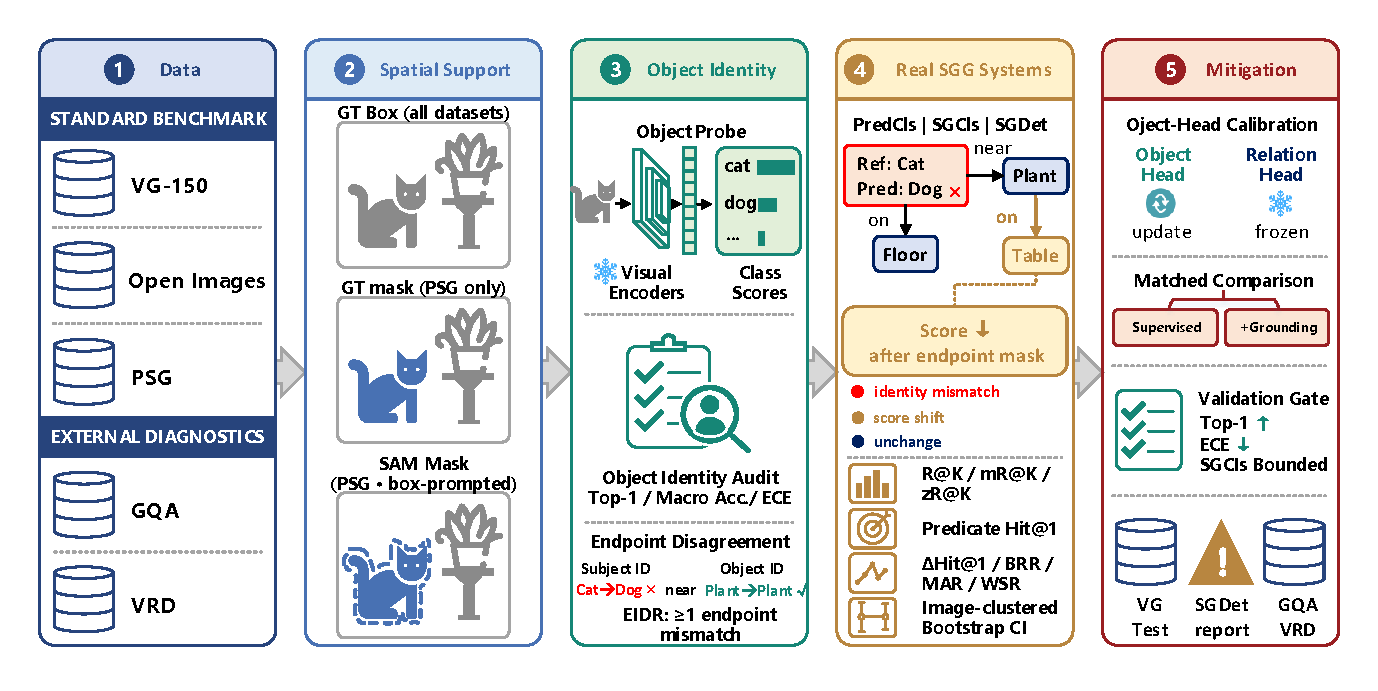
\includegraphics[width=0.98\textwidth]{benchmark_overview.pdf}
  \caption{Overview of \textsc{GroundedSGG-Bench}. Stage 1 separates native
  evaluation on VG-150, Open Images, and PSG from exact-overlap transfer
  diagnostics on GQA and VRD. Stage 2 fixes spatial support with ground-truth
  boxes on all datasets and compares ground-truth and box-prompted SAM masks on
  PSG. Stage 3 probes frozen visual features for object identity and reports
  Top-1, macro accuracy, ECE, and endpoint identity disagreement (EIDR, at
  least one endpoint label differs). Stage 4 evaluates real SGG checkpoints
  under PredCls, SGCls, and SGDet using R/mR/zR, predicate Hit@1,
  endpoint-agreement strata, controlled interventions, and image-clustered
  confidence intervals. Stage 5 updates only the object head while freezing
  relation parameters, applies a validation-only gate, and reports the selected
  state on full VG test and frozen GQA/VRD transfer.}
  \Description{Five-stage benchmark pipeline covering dataset roles, spatial
  support, object-identity probes, real scene-graph systems, and task-focused
  object-head mitigation. Each stage names its inputs, metrics, and claim
  boundary.}
  \label{fig:overview}
\end{figure*}

Our contributions are:
\begin{itemize}
\item \textbf{A claim-scoped benchmark.} We separate support-conditioned identity, relation reasoning under oracle identity, complete-system performance, identity--relation coupling, and mitigation. Every component states what its evidence can and cannot support.
\item \textbf{Executable data and model contracts.} Five dataset entry points use deterministic manifests and ontology hashes. A model is admitted only with checkpoint provenance, score semantics, compatible outputs, and a task-matched reference audit.
\item \textbf{Controlled identity--relation diagnostics.} Dose--response and motif-conditioned audits compare endpoint removal with random, unrelated, appearance-preserving, on-manifold, and matched non-endpoint controls. Results include support, coverage, clean-prediction strata, and image-clustered confidence intervals.
\item \textbf{A closed mitigation study.} TDE-Motifs is evaluated under matched supervised and grounding modes over three seeds. Relation parameters are frozen, selection is validation-only, and selected states are tested on VG and exact-overlap GQA/VRD subsets. This design separates object-head calibration gains from the unsupported claim of an additional grounding benefit.
\end{itemize}

The benchmark is intentionally conservative: prediction caches can establish standard-metric coverage but cannot count as live evidence for interventions or training. Correlation and mediation analyses are descriptive unless the intervention itself identifies a causal contrast.

\section{Benchmark Specification}
\label{sec:design}

\subsection{Scope and claim ladder}

For image $I$, a scene graph is $G=(V,E)$ with entity $v_i=(b_i,m_i,c_i)$, where $b_i$ is a box, $m_i$ an optional mask, and $c_i$ an object class. A directed edge $e_{ij}=(i,p,j)$ assigns predicate $p$ to an ordered pair. A model produces scored triplets $\hat{t}=(\hat b_s,\hat c_s,\hat p,\hat b_o,\hat c_o,q)$.

The benchmark follows a claim ladder. A higher rung may use evidence from lower rungs, but not conversely:
\begin{enumerate}[leftmargin=*]
\item \textbf{Support-conditioned identity:} given a correct box or mask, can frozen features identify the object?
\item \textbf{Relation-side dynamics:} with oracle boxes and labels, how does reasoning alter relation representations and PredCls performance?
\item \textbf{Identity--relation coupling:} when endpoint evidence is perturbed while labels and unrelated nodes are controlled, how do relation predictions change?
\item \textbf{Complete-system validity:} do the same findings coexist with standard PredCls, SGCls, and SGDet performance from real checkpoints?
\item \textbf{Actionability:} can task-focused object calibration improve identity while satisfying a declared task-specific compatibility boundary?
\end{enumerate}

Table~\ref{tab:benchmark-components} maps the executable stages to these claims. Experiment I-B is a secondary diagnostic; it cannot replace I-A, IV, or V.

\begin{table*}[t]
\caption{GroundedSGG-Bench components and claim boundaries. ``Live'' requires
an adapter that recomputes outputs after an intervention; a prediction cache is
insufficient.}
\label{tab:benchmark-components}
\centering
\footnotesize
\begin{tabularx}{\textwidth}{l>{\raggedright\arraybackslash}X>{\raggedright\arraybackslash}X>{\raggedright\arraybackslash}X>{\raggedright\arraybackslash}X}
\toprule
Stage & Question & Data / model requirement & Primary outputs & Claim boundary \\
\midrule
I-A & Does accurate support imply decodable object identity? & PSG; six frozen backbones; box, GT-mask, box-prompted SAM views & Top-1/5, macro, head/body/tail, ECE, high-IoU endpoint disagreement & Scoped to GT-box-prompted support and object probes \\
I-B & How does relation depth change fixed features? & VG-150 PredCls component model & R/mR/zR, effective rank, Dirichlet energy & Relation-only scope under GT object labels \\
II-A & How does predicate accuracy vary with endpoint-label agreement? & Full official prediction caches on VG, OI, and PSG & Hit@1 by endpoint-agreement stratum; support, coverage, and CI & Observational association only \\
II-B & Do targeted endpoint interventions alter relation predictions? & Motifs and Transformer; five strengths; matched controls & Dose--response Hit@1 and matched-control contrasts & Intervention-specific, not a universal causal model \\
III & Do frequent motif predictions persist after endpoint evidence is removed? & Motifs and Transformer; train-mined motifs; GT relation pairs & PIR, clean-correct MAR, clean-wrong WSR, matched-control deltas & Motif-conditioned intervention; no full causal identification \\
IV & Are standard and grounding metrics reproducible across families? & Broad native SGDet panel; two-family matched VG tri-task panel & PredCls/SGCls/SGDet R/mR/zR; decomposition & Breadth and matched-depth results are separate \\
V & Can task-focused object calibration improve identity without harming relations? & TDE-Motifs; two modes; three seeds; frozen relation head & Object Top-1/ECE, SGCls compatibility, full selected-checkpoint test, GQA/VRD transfer & One-family mitigation; grounding benefit is tested against its control \\
\bottomrule
\end{tabularx}
\end{table*}

\subsection{Support-conditioned object identity (Stage I-A)}

PSG provides object masks and a fixed 133-class ontology. For each entity, we extract frozen features under three spatial supports: box ROI pooling, ground-truth-mask pooling, and predicted-mask pooling. Predicted masks are generated by SAM from the ground-truth box. This oracle box prompt isolates mask shape quality from proposal and box-detection variation; we report it specifically as GT-box-prompted segmentation rather than autonomous segmentation.

A linear object classifier is trained separately for every backbone, view, and seed. Images are disjoint across train, validation, and evaluation partitions. Validation controls early stopping and fits one scalar temperature for calibration; the evaluation partition is touched once. We report both all-class metrics and a seen-class subset because an evaluation class with no positive probe-training example is an open-set event, not evidence that the linear probe failed to learn a supported class. Features are cached and remain fixed across probe seeds. Each feature dimension is standardized using statistics fitted only on the probe-training partition and then applied unchanged to validation and evaluation. Every probe uses a 500-epoch cap, patience 20, and minimum validation-loss improvement $10^{-5}$. All 54 backbone--view--seed probes stop early; SAM converges later than the other backbones, with selected epochs 111--136.

For relation endpoint analysis, a relation is eligible at threshold $\tau$ only when both subject and object predicted masks satisfy $\operatorname{IoU}(m,\hat m)\ge\tau$. The endpoint identity disagreement rate is the fraction for which at least one predicted endpoint class differs from its reference label. Reporting support and coverage at every $\tau$ prevents a small high-IoU subset from appearing more conclusive than it is.

\subsection{Identity--relation coupling (Stage II)}

Experiment II-A is an observational audit over complete official prediction caches. It stratifies localized, evaluable ground-truth relations by whether both endpoint identities match their reference labels, exactly one differs, or both differ. It reports predicate Hit@1, relation support, eligibility coverage, and image-clustered bootstrap intervals. Because endpoint agreement is not randomized, II-A can establish association but not a causal effect.

Experiment II-B applies five strengths $\alpha\in\{0,.1,.25,.5,1\}$ to Neural Motifs and an SGG Transformer. The pair represents recurrent contextual reasoning and transformer reasoning under the same VG ontology and split. The primary intervention masks the visually relevant key node or replaces its feature with an on-manifold feature from a matched class/frequency stratum. Controls include a random node, an unrelated node outside the evaluated pair, and mild label-preserving image appearance changes. Object labels, graph indexing, and evaluation triplets are held fixed unless the intervention explicitly targets identity predictions.

\subsection{Motif-conditioned terminal audit (Stage III)}

Stage III mines the 20 most frequent subject--predicate--object motifs from the registered VG training split only, with minimum training support 20, and evaluates all eligible instances in the 2,000-image diagnostic split. The live SGCls adapters are called with ground-truth relation pairs, and the previous pair cap is disabled. For each selected pair, terminal evidence is removed inside the endpoint's ground-truth box using the per-image channel mean. Ground-truth boxes, object labels, relation pairs, relation labels, and graph topology remain fixed. The matched negative control masks the closest-area deterministic non-endpoint box while applying the same selected-pair union-feature ablation. This contract tests endpoint-specific prediction persistence; it does not model every possible intervention or identify a general causal graph.

\subsection{Standard systems and mitigation (Stages IV--V)}

Stage IV separates model breadth from matched task depth. The breadth panel uses provenance-validated native SGDet outputs from recurrent, tree, graph, debiasing, and transformer families across VG, OI, and PSG. The matched-depth panel evaluates Neural Motifs and an SGG Transformer on PredCls, SGCls, and SGDet under one VG ontology and split. This avoids requiring every historical repository to support tasks it did not release while preserving a controlled classic-versus-transformer comparison. Cache-only models broaden standard evaluation but do not silently increase live intervention coverage.

Experiment V is a one-family mitigation study on TDE-Motifs. It compares a task-focused supervised control with a grounding variant for seeds 17, 23, and 31. Both modes update only the object head: relation parameters are frozen, the object loss weight is 2.25, task-focused objects receive weight 3.0, and object weight/bias updates are scaled by 1.1/0.5. We use learning rate $3\times10^{-5}$, 5,000 training images, a disjoint 1,000-image validation split, a five-epoch cap, a three-epoch minimum, and patience one. The strict validation gate requires an object Top-1 gain of at least 0.5 points, no ECE increase above one point, and no SGCls mR@50 decrease above 0.5 points. No test result enters selection. The selected states are frozen and evaluated without adaptation on exact VG-150 label overlaps in GQA and VRD. We report retained image, object, and relation coverage and describe this as a GT-box SGCls-aligned transfer diagnostic rather than native GQA/VRD SGDet.

\section{Benchmark Assets and Governance}
\label{sec:data}

\subsection{Dataset collection and roles}

GroundedSGG-Bench is a benchmarking collection over five existing resources, not a redistribution of their images. VG-150, OI, and PSG form the standard benchmark; GQA and VRD are external diagnostics. Table~\ref{tab:datasets} states each role explicitly. This distinction prevents a model evaluated on an external diagnostic subset from being counted as a native cross-dataset SGG system.

\begin{table*}[t]
\caption{Dataset roles. Ontologies remain dataset-local. ``Support'' describes
the annotation consumed by this benchmark, not every annotation available in
the upstream resource.}
\label{tab:datasets}
\centering
\footnotesize
\begin{tabularx}{\textwidth}{l>{\raggedright\arraybackslash}X>{\raggedright\arraybackslash}X>{\raggedright\arraybackslash}X>{\raggedright\arraybackslash}X>{\raggedright\arraybackslash}X}
\toprule
Dataset & Benchmark role & Spatial support & Relation vocabulary & Main tasks & Primary reason \\
\midrule
VG-150 \cite{krishna2017visual} & Main standard & boxes & 50 predicates & PredCls/SGCls/SGDet & Established closed-vocabulary comparison \\
Open Images \cite{kuznetsova2020openimages} & Native standard & boxes & native OI-SGG & SGDet & Independently collected standard evaluation \\
PSG \cite{yang2022psg} & Main grounding/panoptic & panoptic masks + boxes & 56 predicates & object probe, SGDet & Direct box--mask support comparison \\
GQA \cite{hudson2019gqa} & Annotation-shift diagnostic & boxes & native normalized graph & I-A zero-shot; V frozen transfer & Dense graphs over VG imagery \\
VRD \cite{lu2016vrd} & Independent external diagnostic & boxes & 70 predicates & I-A zero-shot; V frozen transfer & Independent compact relationship corpus \\
\bottomrule
\end{tabularx}
\end{table*}

The VG loader accepts only the canonical VG-SGG HDF5 and dictionary pair, retains the 150-object/50-predicate ontology, and uses the official split field. Open Images uses its released MIDs and relationship descriptions; every MID must resolve in the declared class table. PSG object and predicate category arrays are read from the annotation file, with excluded IDs preserved. GQA normalization is deterministic and recorded in its manifest. VRD uses the released 100-object/70-predicate JSON ontology.

\subsection{Data standardization, ontologies, and splits}

Each run records: absolute logical dataset name, upstream annotation filenames, file sizes and SHA-256 hashes, ontology names and ordered labels, split value, selected image IDs, missing or invalid images, and preprocessing version. The ontology identifier is a digest of the ordered object and predicate lists. A model can run only when its manifest declares the same ontology identifier or a reviewed explicit mapping. This blocks a common silent error in which integer class IDs have plausible ranges but different meanings.

Raw-image readiness is exact for the selected sample, not inferred from folder size. Images are opened and decoded during preflight; GIF/JPEG extension mismatches are resolved by content-aware lookup and then recorded. Deterministic selection skips unavailable images but fails the strict contract when the requested count cannot be met. The formal VG standard run uses the complete 26,446-image test split. Smaller subsets are labeled as smoke or diagnostic runs and cannot populate the headline benchmark table.

Zero-shot triplets are derived solely from the formal training split and saved as an ontology-bound seen-triplet manifest. No evaluation relation contributes to this construction. Probe validation images, early-stopping decisions, and hyperparameter selection are likewise separated from final evaluation images.

\subsection{Model panel and admission protocol}

The benchmark distinguishes a literature taxonomy from an executed model panel. Discussing ten model families does not imply that ten checkpoints were reproduced. A run enters a standard-metric coverage table only after passing the following asset and protocol checks:
\begin{enumerate}[leftmargin=*]
\item repository URL and immutable source commit;
\item checkpoint path, SHA-256 digest, and parameter count;
\item dataset, split, ordered ontology digest, and task;
\item score semantics (logits, categorical probabilities, or independent predicate probabilities) and exact triplet-ranking rule;
\item a complete prediction cache with no missing or duplicate image IDs.
\end{enumerate}

Reference reproduction is reported as a separate task-level status. When a checkpoint-compatible reference exists for the evaluated task, every required reference metric must fall within its predeclared tolerance for the run to be labeled reproduced. When no reference exists for the same checkpoint, task, split, and evaluator, the status is ``not applicable''; the row may document metric coverage but does not enter the reference-pass count. A declared reference that falls outside tolerance is a failure and is excluded from paper-eligible result tables. References for tasks not requested in a run are not evaluated and cannot turn that run into a failure.

Released prediction caches are acceptable for Stage IV standard metrics when provenance and coverage pass. They are rejected for Stages II-B and V because a cache cannot respond to a visual intervention or gradient. Similarly, a repository checkout or downloaded weight is an asset, not a model integration.

The formal model contract has two tiers. First, the native SGDet breadth panel requires at least five architecture families overall, at least five on VG, and at least two each on OI and PSG. Second, the VG matched-depth panel requires complete PredCls, SGCls, and SGDet predictions from Neural Motifs and SGG Transformer over all 26,446 test images. Released RelTR, SGTR, EGTR, KERN, BGNN, VCTree, PSGTR, and PSGFormer artifacts enter the breadth panel only in their supported tasks and ontologies. Both depth models support the live intervention audit; Stage V narrows mitigation to TDE-Motifs so that all registered modes and seeds can be completed under one fixed protocol.

The frozen Stage I-A panel contains ResNet-50, DINOv2-B, SigLIP2-B, RADIOv2.5-B, C-RADIOv4-So400M, and SAM ViT-B. It samples supervised, self-supervised, vision--language, distilled multi-teacher, and segmentation-oriented representations. It is a controlled probe of representation objectives, not an exhaustive foundation-model leaderboard.

\subsection{Artifact schema, access, and maintenance}

The benchmark releases code, manifests, ontology tables, model-adapter schemas, metrics, and derived prediction files where upstream terms permit. It does not rehost VG, COCO/PSG, GQA, OI, or VRD images. Download scripts point to upstream sources and require users to accept their terms. SAM masks are distributed as derived per-image arrays only if the PSG/COCO terms permit; otherwise the deterministic generation script and mask manifest are released.

Every result JSON links to its data manifest and model manifest. Prediction caches store image ID, boxes or masks, entity scores, predicate scores, relation pairs, ontology ID, task, score semantics, and producer version. This provenance-first format is a substantive part of the benchmark: without it, scores from categorical-softmax, independent-sigmoid, and focal-logit models can be inadvertently normalized into different ranking problems.

All formal learning runs use seeds 17, 23, and 31. The reference hardware is two 24-GB RTX 3090 GPUs; per-image batch size and gradient accumulation are recorded separately so the effective batch is reproducible. Automatic mixed precision, library versions, CUDA runtime, preprocessing resolution, ROI chunk size, and evaluation chunk size are stored in each run manifest.

The artifact tree separates raw data, derived features, checkpoints, logs, manifests, and experiment outputs. Every formal command writes a unique run ID, a resolved argument file, environment snapshot, data manifest, model manifest, per-image sufficient statistics, aggregate JSON, and completion marker. A single readiness command checks data coverage, foundation weights, official model assets, task coverage, and live intervention capabilities before GPU execution. Documentation records provenance, intended use, known limitations, and maintenance rather than exposing files without context \cite{gebru2021datasheets}.

Upon acceptance, code and permitted data-derived artifacts will be deposited in an archival repository with a DOI. The release will include environment locks, download and verification scripts, smoke tests, formal commands, and machine-readable tables; upstream images remain under their original terms.

\section{Evaluation Protocol}
\label{sec:metrics}

\subsection{Standard SGG metrics}

For each image, predictions are ranked globally by triplet score; the evaluator does not grant a separate top-$K$ budget to every object pair. We report $K\in\{1,5,10,20,50,100\}$ throughout. A PredCls match requires exact subject, predicate, and object labels on the supplied pair. SGCls additionally requires the predicted endpoint labels on the supplied boxes. SGDet requires label agreement and IoU at least 0.5 for both predicted endpoint boxes. Panoptic mask-IoU results are reported in a separate native-PSG column and are never presented as box-IoU reproduction.

Recall is
\begin{equation}
 R@K=\frac{1}{N}\sum_{i=1}^{N}
 \frac{|\mathcal{T}_i\cap\hat{\mathcal{T}}_{i,K}|}{|\mathcal{T}_i|},
\end{equation}
where $\hat{\mathcal{T}}_{i,K}$ is the image-level top-$K$ set. Mean Recall computes recall independently for each foreground predicate and averages across predicates with evaluation support. Zero-shot Recall restricts the denominator to triplets absent from the ontology-locked training manifest. We publish the supported-class count with mR and the eligible-triplet count with zR.

\subsection{Object identity metrics}

Experiment I-A reports Top-1 and Top-5 accuracy, macro accuracy over supported classes, and head/body/tail accuracy using frequency strata fixed from the probe training partition. Expected calibration error (ECE) uses fixed confidence bins after validation-fitted scalar temperature scaling and is accompanied by accuracy; a low ECE for an inaccurate model is not interpreted as good recognition. Results are reported for all evaluation objects and the training-seen class subset. PSG is the primary mask-conditioned supervised-probe protocol. GQA and VRD add a separate box-only zero-shot SigLIP2 audit in each dataset's native object vocabulary; no classifier or foundation parameter is fitted, training annotations determine frequency strata only, and its uncalibrated zero-shot ECE is not directly compared with PSG's validation-temperature-scaled ECE.

For mask quality threshold $\tau$, let $\mathcal{E}_\tau$ be the relation set whose subject and object masks both have IoU at least $\tau$. Endpoint Identity Disagreement Rate is
\begin{equation}
 \mathrm{EIDR}(\tau)=\frac{1}{|\mathcal{E}_\tau|}
 \sum_{(s,o)\in\mathcal{E}_\tau}
 \mathbb{1}[\hat c_s\ne c_s\ \lor\ \hat c_o\ne c_o].
\end{equation}
We report $|\mathcal{E}_\tau|$ and its fraction of all evaluated relations.

\subsection{Controlled intervention metrics}

For a valid pair-level intervention, Bias-Recall Ratio at $K$ is
\begin{equation}
 \mathrm{BRR}@K=\frac{R@K_{\mathrm{pert}}}{R@K_{\mathrm{clean}}}.
\end{equation}
A high BRR means correct predictions survive removal of targeted evidence; it does not by itself prove that the model uses a particular semantic prior. BRR is undefined when clean recall or relation support falls below the registered minimum. We report each intervention separately before any aggregate.

For Stage III, Prediction Invariance Rate (PIR) is the fraction of all eligible motif instances whose top-1 predicate is unchanged after terminal removal. Motif Association Rate (MAR) applies the same test only to clean-reference-matching predictions, whereas Wrong-prediction Stability Rate (WSR) conditions on clean predictions that differ from the reference. We also report terminal-minus-matched-control differences for each rate. A negative difference means that endpoint removal preserves fewer predictions than non-endpoint removal. This decomposition prevents a high PIR driven by initially wrong predictions from being interpreted as persistence of correct relational evidence.

Physical Violation Rate (PVR) checks only predicates covered by a conservative 2D mutex library and only pairs for which the inverse-direction test is defined:
\begin{equation}
 \mathrm{PVR}=\frac{n_{\mathrm{violations}}}{n_{\mathrm{checked}}}.
\end{equation}
PVR is reported as undefined rather than zero when $n_{\mathrm{checked}}$ is below the minimum. Every PVR value is accompanied by \texttt{pvr\_checked}, coverage, and a confidence interval.

\subsection{Statistical analysis}

The image is the resampling unit. For perturbation experiments, intervention seeds are first averaged within image; a cluster bootstrap then resamples images with replacement to form 95\% percentile intervals. Training comparisons use paired seeds when initialization and data order are matched. We report the bootstrap interval for metric differences, not overlapping marginal intervals as a significance test.

Cross-model analyses are restricted to results sharing a dataset, task, ontology, and endpoint definition. Stage III persistence rates are not pooled with Stage V because mitigation checkpoints do not rerun the motif audit. Mediation language is used only when intervention, mediator, and outcome meet the stated temporal and identification assumptions; otherwise the manuscript says ``association'' and reports the controlled contrast directly.

\section{Benchmark Findings}
\label{sec:results}

\subsection{Spatial support and linearly decodable identity are complementary}

The support-conditioned identity task (Stage I-A) trains image-disjoint linear probes on 65,102 PSG training objects and evaluates 11,667 objects from 1,000 test images. All 133 evaluation classes occur in training. The box-prompted SAM masks have mean IoU 0.713 (median 0.787) against the ground-truth masks. Table~\ref{tab:exp1a} and Figure~\ref{fig:exp1a} report three probe seeds; ``SAM mask'' always denotes a mask predicted from the ground-truth box prompt, not autonomous segmentation.

Mask pooling improves Top-1 accuracy for every encoder. Ground-truth masks add 3.4--9.3 points over boxes, and box-prompted SAM masks add 1.9--4.0 points; every backbone--seed paired image-bootstrap interval for either gain excludes zero. Better support therefore improves identity decodability, but does not remove identity error. Among the 1,511 relations (23.5\% of test relations) for which \emph{both} predicted endpoint masks have IoU $\geq0.85$, at least one predicted endpoint identity differs from the reference in \keynum{13.6--58.5\%} of cases, depending on the frozen backbone. The seed-wise image-bootstrap envelopes are 10.6--17.0\% for C-RADIOv4 and 54.2--63.1\% for ResNet-50. The gap between micro Top-1 and macro accuracy is especially large for SAM ViT-B (58.24\% versus 39.51\%) and ResNet-50 (41.66\% versus 30.65\%), illustrating why aggregate accuracy is accompanied by class-balanced reporting. I-A establishes the first link in the benchmark's evidence chain: conditional spatial support and linearly decoded endpoint identity are distinct measurement dimensions. It does not evaluate autonomous segmentation or identity information recoverable by a nonlinear or end-to-end classifier; Stages II and IV examine complete-system behavior.

The external I-A extension evaluates the same frozen SigLIP2 checkpoint on GT-box crops from 1,000 GQA validation graphs and the complete 955-image VRD test set, using each native object vocabulary and no fitted classifier. On GQA's 1,536-class vocabulary, Top-1 is 16.31\% (image-bootstrap 95\% CI 15.68--16.99\%) and EIDR is 96.62\% (96.14--97.03\%); on VRD's 100-class vocabulary, Top-1 is 49.70\% (48.57--50.98\%) and EIDR is 78.47\% (76.69--80.21\%). GQA is an annotation shift over VG imagery, whereas VRD supplies independently collected images. The values are reported in a separate tier because the vocabularies differ and neither dataset provides the PSG mask-conditioned protocol; they are evidence of external endpoint-identity difficulty, not a cross-dataset model ranking.

\begin{table*}[t]
\caption{Experiment I-A on PSG (\%, mean $\pm$ standard deviation over three probe seeds). ECE follows validation-fitted temperature scaling. SAM mask is ground-truth-box prompted. Endpoint identity disagreement is conditioned on both predicted endpoint masks having IoU $\geq0.85$; support is 1,511 relations with 23.5\% coverage. All probes stop early under the same standardized-feature protocol.}
\label{tab:exp1a}
\centering
\footnotesize
\begin{tabular}{lccccc}
\toprule
Backbone & Box Top-1 & SAM-mask Top-1 & SAM-mask macro & SAM-mask ECE & Endpoint disagreement \\
\midrule
C-RADIOv4 & \keynum{$77.95\pm0.13$} & \keynum{$81.17\pm0.04$} & \keynum{$76.27\pm0.15$} & \keynum{$2.63\pm0.22$} & \keynum{$13.57\pm0.55$} \\
DINOv2-B & $75.51\pm0.10$ & $79.05\pm0.10$ & $72.92\pm0.22$ & $2.74\pm0.10$ & $17.12\pm0.19$ \\
RADIOv2.5-B & $72.88\pm0.13$ & $76.75\pm0.11$ & $69.69\pm0.16$ & $3.21\pm0.15$ & $17.69\pm0.33$ \\
SigLIP2-B & $62.52\pm0.08$ & $66.47\pm0.17$ & $58.36\pm0.14$ & $5.20\pm0.08$ & $23.91\pm0.14$ \\
SAM ViT-B & $54.66\pm0.08$ & $58.24\pm0.03$ & $39.51\pm0.16$ & $4.51\pm0.04$ & $48.80\pm0.31$ \\
ResNet-50 & $39.77\pm0.13$ & $41.66\pm0.20$ & $30.65\pm0.14$ & $12.11\pm0.27$ & \keynum{$58.48\pm0.77$} \\
\bottomrule
\end{tabular}
\end{table*}

\begin{figure}[t]
  \centering
  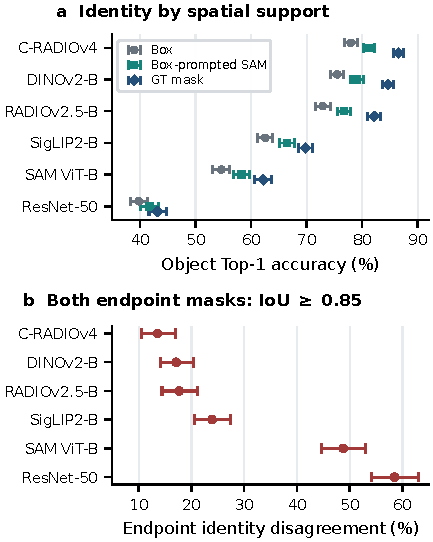
\includegraphics[width=\columnwidth]{experiment1a_identity_grounding.pdf}
  \caption{Experiment I-A. (a) Object Top-1 under box, box-prompted SAM-mask,
  and GT-mask support. (b) Endpoint identity disagreement when both prompted
  masks have IoU $\geq0.85$. Bars are envelopes of seed-wise image-bootstrap
  95\% intervals.}
  \Description{Two-panel dot plot comparing object Top-1 accuracy under box,
  box-prompted SAM mask, and ground-truth mask support, followed by endpoint
  identity disagreement under high mask IoU.}
  \label{fig:exp1a}
\end{figure}

\subsection{Relation-depth diagnostic under oracle identity}

Experiment I-B is complete for six frozen backbones, four GCN depths, and three seeds on VG-150 PredCls. Adding two relation layers improves mR@50 for every backbone: the gain over depth zero ranges from \keynum{0.36} points for RADIOv2.5-B to \keynum{1.30} points for SAM ViT-B. The best depth varies by backbone. Mean mR@50 peaks at depth two for SAM, depth four for C-RADIOv4 and ResNet-50, and depth eight for DINOv2-B, RADIOv2.5-B, and SigLIP2-B; effective rank contracts after its shallow peak. This supports a limited claim about relation-side representation depth. Because PredCls supplies ground-truth object labels, its scope is relation reasoning under supplied identity rather than object recognition. Complete curves are reported in Appendix~\ref{app:formal-results}.

\subsection{Standard-system reproduction}

The completed Experiment IV standard panel contains \keynum{11} full-split SGDet runs spanning \keynum{nine} families and three native ontologies. Seven runs pass their declared task-compatible reference checks. The four PSG caches have no directly comparable checkpoint reference under the evaluated protocol, so their reproduction status is \emph{not applicable} rather than pass or fail. Nine runs also export the object-level records needed for the grounding decomposition in Appendix Table~\ref{tab:app-exp4-grounding}; KERN and BGNN contribute standard SGG metrics in Appendix~\ref{app:formal-results} but are absent from that decomposition because their exported records do not support the same matching audit. Results are grouped by dataset because VG, OI, and PSG use different ontologies, image splits, and prediction protocols. They measure benchmark breadth, not a cross-dataset leaderboard.

The matched-depth VG panel is also complete over all 26,446 test images. The corrected PySGG Transformer evaluation obtains PredCls R/mR@50 of 65.12/17.15 versus registered references of 65.55/16.30. Its SGCls R/mR@50 is 39.39/9.28 versus 40.18/10.09, and its SGDet result is 28.88/7.26 versus 33.04/8.13. PredCls and SGCls lie within the two-point reproduction tolerance for both metrics; only SGDet R@50 remains outside, by \keynum{4.16} points. PySGG Motifs obtains PredCls R/mR@50 of 63.71/18.68, SGCls 28.57/5.82, and SGDet 14.39/2.31. Its PredCls R@50 is within tolerance, but the higher PredCls mR@50 is 3.89 points outside the symmetric reproduction band and the downstream SGCls/SGDet gaps are larger. We retain both provenance-validated checkpoints as live diagnostic baselines, but do not label either complete tri-task run an exact reference reproduction. Full R/mR/zR curves and reference deltas are in Appendix~\ref{app:formal-results}.

\subsection{Predicate accuracy varies with endpoint agreement (Stage II-A)}

Stage II-A is complete as an observational audit of official prediction caches (Appendix Figure~\ref{fig:exp2-propagation}). For three VG SGDet caches evaluated on all 26,446 test images, predicate Hit@1 is 73.2\% versus 63.6\% for EGTR, 73.1\% versus 64.3\% for KERN, and 52.6\% versus 42.2\% for SGTR in the both-match and one-different endpoint strata, respectively; the between-stratum differences are \keynum{8.9--10.4} points. In the both-different stratum, the corresponding values are 49.1\%, 52.6\%, and 36.3\%. The three SGDet audits contain 56,597, 111,849, and 32,371 evaluable relations, corresponding to 30.8\%, 60.9\%, and 17.6\% eligibility coverage. A separate KERN SGCls audit, where ground-truth boxes are supplied, shows the same ordering: 72.1\%, 57.9\%, and 42.2\% across the three endpoint-agreement strata.

The external datasets expose important heterogeneity. OI/EGTR is nearly flat at 87.4\% and 87.2\% in the both-match and one-different strata, whereas OI/SGTR records 67.8\% and 58.8\%; the latter contains only 469 evaluable relations and 9.5\% coverage. On PSG, the corresponding Motifs values are 54.3\% and 41.9\%, and the VCTree values are 54.2\% and 46.7\%. Their both-different estimates are 55.2\% and 56.7\%, but these groups contain only 67 and 60 relations and have wide intervals. Thus endpoint agreement and predicate accuracy are associated on VG, while the direction and magnitude vary across datasets and protocols. Prediction caches do not identify a causal effect.

\paragraph{Controlled live evidence (Stage II-B).} The registered live audit evaluates 1,999 of 2,000 VG images with three intervention seeds per strength. Clean macro-image predicate Hit@1 is 43.00\% for PySGG Motifs and 62.49\% for the corrected PySGG Transformer adapter. At $\alpha=1$, key-node masking reduces Hit@1 by \keynum{23.33} points (95\% CI 21.74--24.83) and \keynum{42.46} points (40.87--44.12), respectively. Random-node masking produces smaller drops of 14.10 and 26.70 points, while unrelated-node masking produces \keynum{5.79} and \keynum{11.54} points. On-manifold replacement yields drops of 17.29 and 30.34 points. Color jitter changes Hit@1 by $-0.23$ points ($-0.81$--0.36) for Motifs and 0.27 points ($-0.05$--0.65) for Transformer, both compatible with zero. The five dose--response strategies and endpoint decomposition completed; pair-recall and physical-consistency subaudits were not rerun, so our claims are restricted to the reported endpoints. The shared ordering across recurrent and transformer adapters provides intervention-specific evidence consistent with II-A, but does not identify a universal causal effect of semantic identity. Exact eligibility, strengths, paired intervals, and SGCls/SGDet endpoint strata are reported in Appendix~\ref{app:formal-results}.

\subsection{Motif persistence is dominated by initially wrong predictions (Stage III)}

The strict Stage III rerun completes for both live adapters with 20 train-mined motifs, 1,411 eligible ground-truth relation pairs, and no evaluation errors. Neural Motifs has 115 clean-correct and 1,296 clean-wrong pairs; the Transformer has 191 and 1,220. Aggregate PIR is 88.87\% (95\% CI 85.66--91.82) for Motifs and 86.18\% (82.17--89.79) for Transformer. This apparent invariance is almost entirely attributable to clean-wrong predictions: WSR is 96.60\% and 99.51\%, whereas clean-correct MAR is only \keynum{1.74\%} (0.00--4.85) and \keynum{1.05\%} (0.00--2.89), respectively.

The matched non-endpoint control sharpens the interpretation. Terminal-minus-control MAR is \keynum{$-51.30$} points (95\% CI $-72.42$ to $-31.24$) for Motifs and \keynum{$-57.89$} points ($-70.57$ to $-43.60$) for Transformer. The corresponding PIR differences are only $-4.26$ and $-5.96$ points because the much larger clean-wrong stratum dominates the aggregate. Thus endpoint removal selectively disrupts initially correct motif predictions; high PIR alone would have supported the opposite and incorrect reading. Appendix Figure~\ref{fig:exp3-motif} visualizes the denominator decomposition and matched-control contrasts. Because each row uses one fixed checkpoint and a deterministic intervention, intervals quantify image-level sampling uncertainty rather than training-seed variation.

\subsection{Task-focused object-head mitigation (Stage V)}

All six registered TDE-Motifs runs reach the three-epoch minimum and stop under the common early-stopping rule (Appendix Table~\ref{tab:app-exp5-vg}). Relative to the shared frozen baseline, the supervised control improves object Top-1 by \keynum{$0.48\pm0.05$} points and the grounding variant by \keynum{$0.50\pm0.01$} points. ECE falls from \keynum{17.87\%} to \keynum{2.68\%} and \keynum{3.22\%}, respectively. SGCls R@50 and mR@50 also increase, which is consistent with updating the object head while freezing relation parameters. The strict gate passes two of three supervised seeds and one of three grounding seeds; the failed seeds miss the 0.5-point object-gain threshold, not the relation-preservation boundary. The experiment supports task-focused object-head calibration, but not a stable incremental benefit from the grounding term.

The frozen exact-overlap transfer follows the same pattern (Appendix
Table~\ref{tab:app-exp5-external}). On GQA, object Top-1 increases by
\keynum{8.59--9.36} points and triplet Hit@1 by \keynum{5.90--6.33}
points; on VRD, the gains are \keynum{6.16--6.33} and
\keynum{1.37--1.42} points. Predicate Hit@1 is unchanged because the
relation head is frozen, while EIDR decreases. Exact-label mapping covers
only 3.47\% of GQA and 31.56\% of VRD relations, so this is a conservative
frozen-transfer diagnostic rather than native cross-dataset SGG.

A selection-independent full VG test of supervised seed 17 preserves the
registered SGCls boundary ($\Delta$mR@50 $=-0.38$) but reduces SGDet
mR@50 by \keynum{6.35} points. Freezing relation parameters does not
protect SGDet because updated object scores still affect labeling and
triplet ranking; full metrics and this claim boundary appear in
Appendix~\ref{app:formal-results}.

\section{Positioning, Limitations, and Ethics}

GroundedSGG-Bench complements contextual, debiased, and end-to-end SGG
\cite{zellers2018motifs,tang2020unbiased,li2022sgtr,cong2023reltr,im2024egtr}.
It does not claim universal causal attribution or preserved detector utility:
PredCls supplies labels, prompted masks provide oracle support, and external
transfer uses exact vocabulary overlap. We redistribute no images. Scene
graphs inherit dataset bias and should not support surveillance or high-stakes
decisions without separate consent, privacy, and fairness review. Extended
positioning, limitations, and resource costs appear in the appendix.

\section{Conclusion}

\textsc{GroundedSGG-Bench} evaluates the path from spatial support to object
identity and relations under explicit claim contracts. Even at prompted-mask
IoU 0.85, endpoint disagreement is \keynum{13.6--58.5\%}. Across \keynum{11}
full-split SGDet runs, endpoint disagreement predicts lower relation accuracy,
while controlled key-node masking reduces predicate Hit@1 by \keynum{23.33}
and \keynum{42.46} points. The motif audit resolves misleading aggregate
invariance: clean-correct persistence is only \keynum{1.05--1.74\%} and trails
a matched control by \keynum{51.3--57.9} points. Task-focused TDE-Motifs
tuning improves object calibration and SGCls-aligned metrics, including on
exact-overlap GQA and VRD subsets, but grounding is not consistently better
than supervised control and the selected checkpoint degrades SGDet. The
benchmark therefore supports separate reporting of localization, identity,
and relation quality rather than a single end-to-end score.

\bibliographystyle{ACM-Reference-Format}
\bibliography{reference}

\appendix
\section{Reproducibility Checklist}

Appendix~\ref{app:formal-results} reports the complete aggregate tables for every currently paper-eligible run. The archival release additionally includes exact commands; environment and package locks; data and checkpoint SHA-256 manifests; model-specific preprocessing; score semantics; reference metrics and tolerances; per-class support; bootstrap seeds; failed-run accounting; and the license/access table for every upstream dataset and checkpoint.

\section{Required Model Manifest Fields}

\begingroup\sloppy Each model manifest contains \path{name}, \path{architecture_family}, \path{paradigm}, \path{repository}, \path{source_commit}, \path{checkpoint}, \path{checkpoint_sha256}, \path{parameter_count}, \path{dataset}, \path{ontology_id}, \path{tasks}, \path{relation_score_mode}, \path{execution_mode}, preprocessing, reference metrics, tolerances, and intervention capabilities. \par\endgroup

\section{Result Eligibility and Failure Reporting}

Smoke and subset runs must contain ``smoke'' or the sample count in their run identifier and cannot populate formal tables. A metric is never replaced with zero because its denominator is empty. Missing support, incomplete image coverage, and ontology mismatch are explicit statuses in JSON and paper tables. Reference checks are scoped to the task requested by the run: a compatible reference is marked pass or fail, an unavailable compatible reference is marked not applicable, and an unrequested task is not evaluated.

\section{Extended Related Work}

\paragraph{Datasets and evaluation.}
VRD introduced zero-shot relationship evaluation \cite{lu2016vrd}; VG supplied the dense annotations behind VG-150 \cite{krishna2017visual}; and message passing established PredCls/SGCls/SGDet \cite{xu2017scene}. OI adds independently collected relationship data, GQA normalizes VG graphs for question answering, and PSG replaces box-only entities with panoptic segments \cite{kuznetsova2020openimages,hudson2019gqa,yang2022psg}. Alongside R@K, mR@K and zR@K expose long-tail and compositional behavior \cite{tang2020unbiased}; recent work further studies unseen-triplet equivariance, conformal coverage, and synthetic completion \cite{huang2025capsgg,nag2025conformal,park2025svg}.

\paragraph{Models and representations.}
Contextual SGG spans Motifs, VCTree, KERN, GPS-Net, BGNN, and TDE \cite{zellers2018motifs,tang2019vctree,chen2019kern,lin2020gpsnet,li2021bgnn,tang2020unbiased}. End-to-end systems use triplet queries, detector attention, dense queries, reciprocal alignment, or semantic--geometric generation \cite{li2022sgtr,cong2023reltr,im2024egtr,hayder2024dsgg,fu2025hrt,hu2026flowsg}. Our frozen panel spans supervised, self-supervised, image--text, multi-teacher, and segmentation representations \cite{he2016resnet,oquab2024dinov2,tschannen2025siglip2,heinrich2025radio25,ranzinger2026cradiov4,kirillov2023sam}; matched-support probes measure identity decodability without assigning an intrinsic grounding label to any backbone.

\paragraph{Identity errors, knowledge, and robustness.}
Graphical contrastive losses explicitly target entity-instance confusion
\cite{zhang2019graphical}; external knowledge and reconstruction address noisy
graph labels \cite{gu2019external}; and counterfactual rewards,
knowledge-graph bridging, and learned visual commonsense promote coherent
predictions
\cite{chen2019counterfactual,zareian2020bridging,zareian2020commonsense}.
Open-vocabulary relation mining, universal label spaces, and
mixture-of-experts decoupling broaden the recognition target
\cite{min2025vlirm,wu2025universal,li2026moefd}, while Robo-SGG studies
corruption robustness \cite{lv2026robosgg}. These methods improve training;
GroundedSGG-Bench instead standardizes the endpoint-grounding measurements
needed to compare their resulting checkpoints.

\paragraph{Agent state and benchmark infrastructure.}
Scene Graph Memory, SayPlan, ConceptGraphs, and GraphEQA expose why identity errors matter when graphs become persistent state \cite{kurenkov2023sgm,rana2023sayplan,gu2024conceptgraphs,saxena2025grapheqa}. H2GB, DCA-Bench, BatteryLife, and the misinformation-evaluation guide similarly treat reproducible data and workflow contracts as benchmark components \cite{lin2025h2gb,huang2025dcabench,tan2025batterylife,thibault2025misinformation}. GroundedSGG-Bench therefore audits asset readiness, ontology alignment, prediction coverage, and evaluator behavior before admitting a numerical result.

\section{Extended Resource, Limitation, and Ethics Statement}

The complete scope and dataset limitations are those summarized in the main paper. The archival release additionally records compute hardware, environments, failed runs, and checkpoint/data access terms. It redistributes neither raw images nor original third-party checkpoints. Frequency-stratified results are not a fairness audit, and all downstream uses require their own privacy, consent, and bias assessment.

\section{Additional Result Visualizations}

\begin{figure}[h]
  \centering
  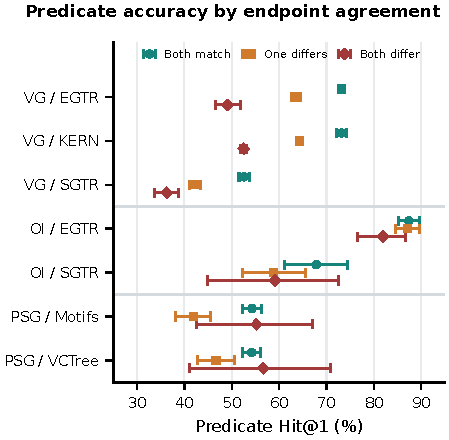
\includegraphics[width=\columnwidth]{experiment2_error_propagation.pdf}
  \caption{Experiment II-A predicate Hit@1 by endpoint-agreement stratum.
  Bars are image-bootstrap 95\% intervals. Rows retain native ontologies; the
  PSG both-different groups have only 67 and 60 relations. These are
  observational associations.}
  \Description{A compact row-wise dot plot compares predicate Hit at one when
  both endpoint identities match, one differs, or both differ for seven
  model--dataset runs.}
  \label{fig:exp2-propagation}
\end{figure}

\begin{figure}[h]
  \centering
  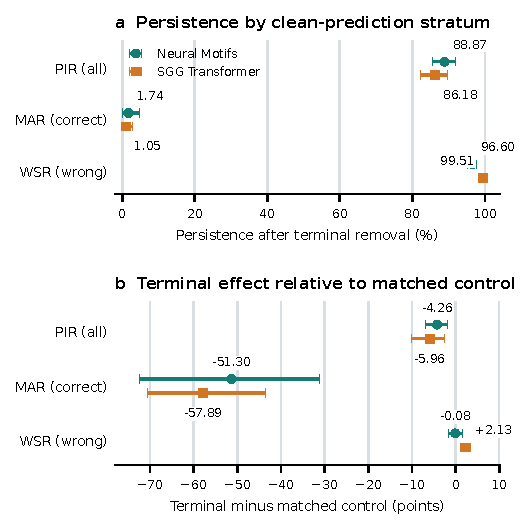
\includegraphics[width=\columnwidth]{experiment3_motif_intervention.pdf}
  \caption{Experiment III motif-conditioned terminal audit. (a) Prediction
  persistence after terminal removal, separated into all pairs (PIR),
  clean-correct pairs (MAR), and clean-wrong pairs (WSR). (b)
  Terminal-minus-matched-control differences; negative values indicate lower
  persistence after endpoint removal. Points show estimates and bars show
  image-bootstrap 95\% intervals.}
  \Description{Two stacked interval plots compare Neural Motifs and an SGG
  Transformer. Overall and clean-wrong predictions are highly stable, but
  clean-correct prediction persistence is near zero and much lower than under
  matched non-endpoint removal.}
  \label{fig:exp3-motif}
\end{figure}

\section{Experiment I-B: Relation-Depth Diagnostic}

Experiment I-B is deliberately secondary to the object-identity evidence. It uses ground-truth boxes and object labels under VG-150 PredCls, and therefore cannot test whether an object is visually recognized. Across six frozen backbones and three seeds, adding two GCN relation layers improves mR@50 over the depth-zero component for every backbone (Figure~A1). Further depth is not uniformly beneficial. Effective rank peaks at depth two and then contracts by depth eight for all six backbones, while mR@50 mostly plateaus. This result supports a limited representation-depth diagnostic, not the paper's main object-grounding claim.

\begin{center}
\centering
  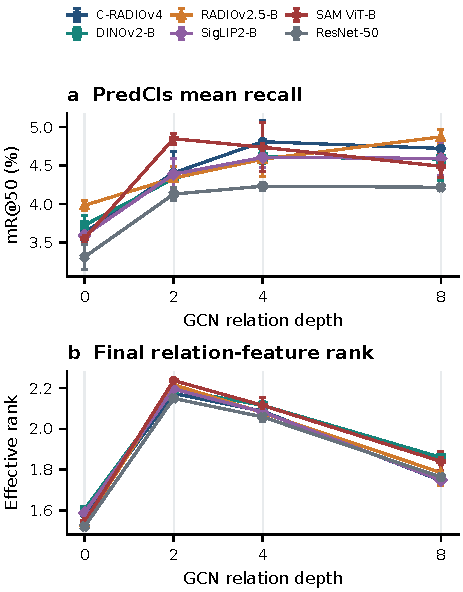
\includegraphics[width=0.94\columnwidth]{experiment1b_depth_diagnostics.pdf}
\par\smallskip \parbox{\columnwidth}{\small\textbf{Figure A1:} Experiment I-B on VG-150 PredCls (mean $\pm$ standard deviation over three seeds). Two relation layers improve mR@50 for every frozen backbone, whereas deeper propagation gives inconsistent utility and lower final-layer effective rank. Ground-truth object labels make this a relation-component study rather than an object-recognition experiment.}
\end{center}

% BEGIN AUTO-GENERATED FORMAL RESULT TABLES
\section{Complete Formal Result Tables}
\label{app:formal-results}

This appendix contains only paper-eligible full, formal, or converged runs. Smoke tests, 100/1,000-image debugging subsets, failed attempts, superseded Experiment~I runs, and duplicate reruns are excluded. Percentages are reported on the 0--100 scale. Native dataset ontologies and task contracts are retained; values from VG, OI, and PSG are not treated as a shared leaderboard.

\begin{table*}[t]
\caption{Formal-result inventory included in this appendix. Completed runs without a checkpoint-compatible reference are reported with reproduction status not applicable.}
\label{tab:app-inventory}
\centering
\footnotesize
\setlength{\tabcolsep}{2.5pt}
\begin{tabular}{lllll}
\toprule
Stage & Dataset/task & Formal scale & Included systems & Appendix tables \\
\midrule
I-A & PSG object probe & 65,102 train / 11,667 eval objects & 6 backbones, 3 views, 3 seeds & \ref{tab:app-exp1a-complete}--\ref{tab:app-exp1a-endpoints} \\
I-B & VG-150 PredCls & 2,000 test images & 6 backbones, 4 depths, 3 seeds & \ref{tab:app-exp1b-r}--\ref{tab:app-exp1b-diagnostics} \\
II-A & VG/OI/PSG observational & Full registered splits & 8 task runs / 7 model--dataset runs & \ref{tab:app-exp2-coverage}--\ref{tab:app-exp2-groups} \\
II-B & VG controlled interventions & 1,999/2,000 images, 3 seeds & Motifs; SGG Transformer & \ref{tab:app-exp2b-dose}--\ref{tab:app-exp2b-endpoints} \\
III & VG motif terminal audit & 20 motifs / 1,411 GT pairs & Motifs; SGG Transformer & \ref{tab:app-exp3-motif} \\
IV & Native SGDet & 26,446/1,813/1,000 images & 11 runs, 9 families; 9 decomposed & \ref{tab:app-exp4-r}--\ref{tab:app-exp4-grounding} \\
IV-depth & VG PredCls/SGCls/SGDet & 26,446 images & Motifs; SGG Transformer & \ref{tab:app-exp4-depth-metrics}--\ref{tab:app-exp4-depth-reference} \\
IV auxiliary & VG-150 SGCls & 26,446 images & KERN & \ref{tab:app-kern-sgcls} \\
V & Object-head mitigation & 5,000 train / 1,000 validation images; 2 modes; 3 seeds & TDE-Motifs & \ref{tab:app-exp5-vg}--\ref{tab:app-exp5-test} \\
V external & Frozen shared-VG transfer & GQA 604/1,000; VRD 770/955 retained images & Six selected TDE-Motifs states & \ref{tab:app-exp5-external} \\
\bottomrule
\end{tabular}
\end{table*}

% Experiment I-A tables
\paragraph{Experiment I-A: support quality does not determine identity.}
Tables~\ref{tab:app-exp1a-complete}--\ref{tab:app-exp1a-endpoints} separate
support type, class frequency, object area, and mask quality. Ground-truth masks
give the strongest recognition for every encoder, and box-prompted SAM masks
usually improve over boxes, but the encoder ordering remains large: SAM-mask
Top-1 ranges from \keynum{41.66\%} for ResNet-50 to \keynum{81.17\%} for
C-RADIOv4. Recognition also improves with mask IoU, yet at the preregistered
IoU threshold of 0.85 the endpoint disagreement rate still spans
\keynum{13.57--58.48\%}. Thus accurate support helps but does not certify the
identity assigned to either endpoint.

\begin{table*}[t]
\caption{Complete Experiment I-A object-probe results on PSG (mean $\pm$ standard deviation over seeds 17, 23, and 31). Accuracy and validation-temperature-scaled ECE are percentages. SAM masks are predicted from ground-truth box prompts.}
\label{tab:app-exp1a-complete}
\centering
\footnotesize
\setlength{\tabcolsep}{2.5pt}
\renewcommand{\arraystretch}{1}
\begin{tabular}{llrrrrrr}
\toprule
Backbone & Support & Top-1 & Top-5 & Macro & ECE & NLL & Brier \\
\midrule
C-RADIOv4 & Box & $77.95\pm0.13$ & $96.05\pm0.02$ & $71.71\pm0.04$ & $3.67\pm0.27$ & $0.826\pm0.001$ & $0.320\pm0.001$ \\
C-RADIOv4 & SAM mask & \keynum{$81.17\pm0.04$} & $96.14\pm0.08$ & \keynum{$76.27\pm0.15$} & $2.63\pm0.22$ & $0.728\pm0.005$ & $0.278\pm0.002$ \\
C-RADIOv4 & GT mask & \keynum{$86.54\pm0.03$} & \keynum{$97.52\pm0.04$} & \keynum{$81.79\pm0.11$} & $1.90\pm0.17$ & \keynum{$0.521\pm0.001$} & \keynum{$0.200\pm0.000$} \\
DINOv2-B & Box & $75.51\pm0.10$ & $95.10\pm0.09$ & $69.09\pm0.11$ & $3.87\pm0.14$ & $0.937\pm0.005$ & $0.354\pm0.002$ \\
DINOv2-B & SAM mask & $79.05\pm0.10$ & $95.51\pm0.04$ & $72.92\pm0.22$ & $2.74\pm0.10$ & $0.806\pm0.001$ & $0.304\pm0.000$ \\
DINOv2-B & GT mask & $84.66\pm0.03$ & $96.92\pm0.02$ & $78.98\pm0.13$ & $1.77\pm0.25$ & $0.600\pm0.003$ & $0.225\pm0.001$ \\
RADIOv2.5-B & Box & $72.88\pm0.13$ & $93.90\pm0.04$ & $65.07\pm0.15$ & $3.66\pm0.16$ & $1.037\pm0.003$ & $0.389\pm0.001$ \\
RADIOv2.5-B & SAM mask & $76.75\pm0.11$ & $94.50\pm0.06$ & $69.69\pm0.16$ & $3.21\pm0.15$ & $0.900\pm0.002$ & $0.337\pm0.001$ \\
RADIOv2.5-B & GT mask & $82.16\pm0.12$ & $96.05\pm0.04$ & $75.32\pm0.16$ & $2.24\pm0.06$ & $0.697\pm0.002$ & $0.263\pm0.001$ \\
SigLIP2-B & Box & $62.52\pm0.08$ & $87.73\pm0.08$ & $54.72\pm0.02$ & $5.95\pm0.15$ & $1.550\pm0.001$ & $0.533\pm0.000$ \\
SigLIP2-B & SAM mask & $66.47\pm0.17$ & $88.26\pm0.04$ & $58.36\pm0.14$ & $5.20\pm0.08$ & $1.441\pm0.003$ & $0.486\pm0.001$ \\
SigLIP2-B & GT mask & $69.80\pm0.06$ & $89.43\pm0.11$ & $61.52\pm0.17$ & $4.90\pm0.16$ & $1.321\pm0.001$ & $0.440\pm0.000$ \\
SAM ViT-B & Box & $54.66\pm0.08$ & $80.74\pm0.02$ & $35.87\pm0.16$ & $4.84\pm0.11$ & $1.914\pm0.001$ & $0.606\pm0.000$ \\
SAM ViT-B & SAM mask & $58.24\pm0.03$ & $81.79\pm0.08$ & $39.51\pm0.16$ & $4.51\pm0.04$ & $1.782\pm0.004$ & $0.562\pm0.001$ \\
SAM ViT-B & GT mask & $62.17\pm0.11$ & $85.07\pm0.03$ & $43.15\pm0.02$ & $4.07\pm0.11$ & $1.600\pm0.002$ & $0.511\pm0.001$ \\
ResNet-50 & Box & $39.77\pm0.13$ & $71.41\pm0.06$ & $29.42\pm0.23$ & $11.13\pm0.14$ & $2.762\pm0.001$ & $0.805\pm0.000$ \\
ResNet-50 & SAM mask & $41.66\pm0.20$ & $71.86\pm0.11$ & $30.65\pm0.14$ & $12.11\pm0.27$ & $2.746\pm0.002$ & $0.792\pm0.001$ \\
ResNet-50 & GT mask & $43.17\pm0.14$ & $72.66\pm0.22$ & $31.88\pm0.20$ & $12.82\pm0.33$ & $2.705\pm0.003$ & $0.782\pm0.000$ \\
\bottomrule
\end{tabular}
\end{table*}

\begin{table*}[t]
\caption{Experiment I-A SAM-mask Top-1 accuracy by training-frequency and object-area strata (\%). Frequency strata are fixed from the probe training partition.}
\label{tab:app-exp1a-strata}
\centering
\footnotesize
\setlength{\tabcolsep}{2.5pt}
\renewcommand{\arraystretch}{1}
\begin{tabular}{lrrrrrr}
\toprule
Backbone & Head & Body & Tail & Small & Medium & Large \\
\midrule
C-RADIOv4 & $79.38\pm0.20$ & $76.22\pm0.58$ & $72.99\pm0.12$ & $83.51\pm0.09$ & $84.72\pm0.21$ & $76.39\pm0.07$ \\
DINOv2-B & $76.26\pm0.20$ & $74.63\pm0.49$ & $67.57\pm0.79$ & $80.37\pm0.14$ & $82.89\pm0.16$ & $75.37\pm0.09$ \\
RADIOv2.5-B & $73.69\pm0.08$ & $70.69\pm0.31$ & $64.35\pm0.26$ & $76.64\pm0.44$ & $80.43\pm0.37$ & $74.88\pm0.18$ \\
SigLIP2-B & $61.99\pm0.13$ & $61.87\pm0.16$ & $50.77\pm0.48$ & $59.51\pm0.18$ & $73.16\pm0.63$ & $71.27\pm0.05$ \\
SAM ViT-B & $50.74\pm0.15$ & $40.22\pm0.28$ & $26.74\pm0.28$ & $58.54\pm0.19$ & $57.75\pm0.15$ & $58.13\pm0.27$ \\
ResNet-50 & $35.86\pm0.53$ & $30.85\pm0.16$ & $24.86\pm0.23$ & $32.00\pm0.40$ & $43.28\pm0.25$ & $52.52\pm0.20$ \\
\bottomrule
\end{tabular}
\end{table*}

\begin{table*}[t]
\caption{Experiment I-A SAM-mask object Top-1 accuracy (\%) by predicted-mask IoU bin. The same 11,667 evaluation objects are partitioned by mask quality.}
\label{tab:app-exp1a-iou}
\centering
\footnotesize
\setlength{\tabcolsep}{2.5pt}
\renewcommand{\arraystretch}{1}
\begin{tabular}{lrrrrr}
\toprule
Backbone & $[0,.50)$ & $[.50,.70)$ & $[.70,.85)$ & $[.85,.95)$ & $[.95,1]$ \\
\midrule
C-RADIOv4 & $47.22\pm0.25$ & $79.33\pm0.15$ & $87.87\pm0.16$ & $91.53\pm0.12$ & $92.52\pm0.08$ \\
DINOv2-B & $45.12\pm0.32$ & $77.09\pm0.44$ & $85.64\pm0.16$ & $89.39\pm0.04$ & $91.62\pm0.21$ \\
RADIOv2.5-B & $43.77\pm0.28$ & $73.51\pm0.36$ & $82.65\pm0.20$ & $87.73\pm0.22$ & $91.57\pm0.14$ \\
SigLIP2-B & $35.67\pm0.26$ & $58.87\pm0.46$ & $70.35\pm0.06$ & $80.05\pm0.19$ & $87.35\pm0.14$ \\
SAM ViT-B & $31.88\pm0.15$ & $53.97\pm0.22$ & $63.82\pm0.12$ & $67.03\pm0.17$ & $70.55\pm0.56$ \\
ResNet-50 & $22.67\pm0.18$ & $32.25\pm0.14$ & $42.26\pm0.42$ & $52.29\pm0.11$ & $69.48\pm0.60$ \\
\bottomrule
\end{tabular}
\end{table*}

\begin{table*}[t]
\caption{Experiment I-A endpoint identity disagreement rate (\%) conditioned on both relation endpoints meeting the stated box-prompted mask-IoU threshold. Supports are 3,012, 1,511, 621, and 60 relations at thresholds 0.75, 0.85, 0.90, and 0.95, respectively.}
\label{tab:app-exp1a-endpoints}
\centering
\scriptsize
\setlength{\tabcolsep}{1.2pt}
\renewcommand{\arraystretch}{0.94}
\begin{tabular}{lrrrr}
\toprule
Backbone & IoU$\geq.75$ & IoU$\geq.85$ & IoU$\geq.90$ & IoU$\geq.95$ \\
\midrule
C-RADIOv4 & $15.31\pm0.35$ & \keynum{$13.57\pm0.55$} & $14.06\pm1.19$ & $12.78\pm0.79$ \\
DINOv2-B & $17.80\pm0.24$ & $17.12\pm0.19$ & $17.12\pm0.38$ & $7.22\pm0.79$ \\
RADIOv2.5-B & $19.77\pm0.23$ & $17.69\pm0.33$ & $17.02\pm0.50$ & $10.56\pm0.79$ \\
SigLIP2-B & $27.14\pm0.11$ & $23.91\pm0.14$ & $21.63\pm0.08$ & $20.00\pm2.72$ \\
SAM ViT-B & $50.80\pm0.28$ & $48.80\pm0.31$ & $49.33\pm0.27$ & $36.67\pm2.36$ \\
ResNet-50 & $63.24\pm0.71$ & \keynum{$58.48\pm0.77$} & $55.82\pm1.33$ & $47.78\pm2.08$ \\
\bottomrule
\end{tabular}
\end{table*}

% Experiment I-B tables
\paragraph{Experiment I-B: shallow relation propagation is sufficient.}
Tables~\ref{tab:app-exp1b-r}--\ref{tab:app-exp1b-diagnostics} report the full
PredCls depth sweep. Moving from depth zero to two improves mR@50 for all six
frozen encoders, whereas the best later depth depends on the backbone and the
gains largely plateau. Effective rank peaks at depth two and contracts by depth
eight for every encoder. Because object labels are supplied, these results
diagnose relation-side representation depth and provide no object-recognition
evidence.

\begin{table*}[t]
\caption{Complete Experiment I-B VG-150 PredCls Recall (\%, mean $\pm$ standard deviation over three seeds). Ranking is image-level and uses one top-$K$ budget per image.}
\label{tab:app-exp1b-r}
\centering
\footnotesize
\setlength{\tabcolsep}{2.5pt}
\renewcommand{\arraystretch}{1}
\begin{tabular}{lrrrrrrr}
\toprule
Backbone & Depth & @1 & @5 & @10 & @20 & @50 & @100 \\
\midrule
C-RADIOv4 & 0 & $2.52\pm0.17$ & $9.45\pm0.10$ & $14.89\pm0.13$ & $22.28\pm0.09$ & $35.08\pm0.05$ & $45.92\pm0.15$ \\
C-RADIOv4 & 2 & $4.02\pm0.11$ & $13.31\pm0.22$ & $19.43\pm0.51$ & $26.71\pm0.17$ & $39.26\pm0.26$ & $49.67\pm0.25$ \\
C-RADIOv4 & 4 & $3.95\pm0.26$ & $13.39\pm0.65$ & $19.99\pm0.65$ & $27.97\pm0.54$ & $40.71\pm0.68$ & $51.63\pm0.69$ \\
C-RADIOv4 & 8 & $3.61\pm0.08$ & $12.57\pm0.36$ & $19.01\pm0.22$ & $27.01\pm0.38$ & $40.22\pm0.53$ & $51.39\pm0.47$ \\
DINOv2-B & 0 & $2.62\pm0.11$ & $9.38\pm0.17$ & $15.05\pm0.28$ & $22.27\pm0.19$ & $35.22\pm0.31$ & $45.70\pm0.12$ \\
DINOv2-B & 2 & $4.03\pm0.11$ & $13.01\pm0.23$ & $19.26\pm0.11$ & $26.34\pm0.22$ & $38.38\pm0.12$ & $48.84\pm0.49$ \\
DINOv2-B & 4 & $4.01\pm0.13$ & $13.30\pm0.24$ & $19.60\pm0.33$ & $27.17\pm0.41$ & $39.36\pm0.47$ & $49.89\pm0.17$ \\
DINOv2-B & 8 & $3.79\pm0.18$ & $12.75\pm0.39$ & $19.37\pm0.60$ & $26.97\pm0.78$ & $39.78\pm0.92$ & $50.64\pm1.04$ \\
RADIOv2.5-B & 0 & $2.80\pm0.18$ & $10.16\pm0.03$ & $15.83\pm0.10$ & $23.87\pm0.14$ & $37.69\pm0.13$ & $49.38\pm0.23$ \\
RADIOv2.5-B & 2 & $4.07\pm0.05$ & $13.48\pm0.21$ & $20.08\pm0.19$ & $27.41\pm0.18$ & $39.50\pm0.10$ & $50.14\pm0.40$ \\
RADIOv2.5-B & 4 & $4.25\pm0.25$ & $13.77\pm0.61$ & $20.29\pm0.86$ & $28.11\pm0.76$ & $40.46\pm0.61$ & $50.48\pm0.89$ \\
RADIOv2.5-B & 8 & $3.99\pm0.01$ & $13.24\pm0.09$ & $19.87\pm0.38$ & $28.32\pm0.15$ & $42.09\pm0.32$ & $53.18\pm0.14$ \\
SigLIP2-B & 0 & $2.47\pm0.11$ & $9.49\pm0.01$ & $15.00\pm0.12$ & $22.11\pm0.06$ & $34.92\pm0.05$ & $45.87\pm0.07$ \\
SigLIP2-B & 2 & $4.15\pm0.10$ & $13.60\pm0.22$ & $19.99\pm0.15$ & $27.10\pm0.25$ & $39.24\pm0.18$ & $49.32\pm0.31$ \\
SigLIP2-B & 4 & $4.06\pm0.14$ & $13.28\pm0.45$ & $19.75\pm0.38$ & $27.38\pm0.43$ & $40.20\pm0.77$ & $50.72\pm0.48$ \\
SigLIP2-B & 8 & $3.75\pm0.20$ & $12.83\pm0.32$ & $19.26\pm0.47$ & $26.86\pm0.39$ & $40.21\pm0.51$ & $51.02\pm0.37$ \\
SAM ViT-B & 0 & $2.36\pm0.06$ & $9.20\pm0.19$ & $15.19\pm0.27$ & $23.10\pm0.36$ & $36.92\pm0.08$ & $49.23\pm0.18$ \\
SAM ViT-B & 2 & $3.98\pm0.28$ & $14.11\pm0.28$ & $21.15\pm0.59$ & $29.43\pm0.22$ & $42.99\pm0.30$ & $54.51\pm0.14$ \\
SAM ViT-B & 4 & $4.08\pm0.13$ & $14.16\pm0.11$ & $21.73\pm0.25$ & $29.90\pm0.74$ & $42.77\pm1.37$ & $53.21\pm2.47$ \\
SAM ViT-B & 8 & $3.83\pm0.26$ & $13.50\pm0.35$ & $20.60\pm0.22$ & $28.93\pm0.16$ & $42.24\pm0.29$ & $52.87\pm0.44$ \\
ResNet-50 & 0 & $2.44\pm0.13$ & $8.51\pm0.17$ & $13.80\pm0.13$ & $21.24\pm0.31$ & $33.29\pm0.38$ & $44.37\pm0.39$ \\
ResNet-50 & 2 & $3.62\pm0.07$ & $12.26\pm0.17$ & $18.10\pm0.21$ & $25.24\pm0.35$ & $37.38\pm0.76$ & $47.57\pm0.83$ \\
ResNet-50 & 4 & $3.43\pm0.10$ & $12.05\pm0.13$ & $18.02\pm0.26$ & $25.62\pm0.24$ & $37.43\pm0.19$ & $47.63\pm0.19$ \\
ResNet-50 & 8 & $3.34\pm0.09$ & $11.71\pm0.51$ & $17.53\pm0.46$ & $25.23\pm0.37$ & $37.36\pm0.46$ & $48.10\pm0.30$ \\
\bottomrule
\end{tabular}
\end{table*}

\begin{table*}[t]
\caption{Complete Experiment I-B VG-150 PredCls mean Recall (\%, mean $\pm$ standard deviation over three seeds). Ranking is image-level and uses one top-$K$ budget per image.}
\label{tab:app-exp1b-mr}
\centering
\footnotesize
\setlength{\tabcolsep}{2.5pt}
\renewcommand{\arraystretch}{1}
\begin{tabular}{lrrrrrrr}
\toprule
Backbone & Depth & @1 & @5 & @10 & @20 & @50 & @100 \\
\midrule
C-RADIOv4 & 0 & $0.15\pm0.03$ & $0.62\pm0.04$ & $1.07\pm0.02$ & $1.85\pm0.04$ & $3.63\pm0.08$ & $5.63\pm0.12$ \\
C-RADIOv4 & 2 & $0.26\pm0.02$ & $1.04\pm0.06$ & $1.64\pm0.09$ & $2.52\pm0.16$ & $4.41\pm0.23$ & $6.73\pm0.17$ \\
C-RADIOv4 & 4 & $0.25\pm0.02$ & $1.04\pm0.07$ & $1.72\pm0.11$ & $2.73\pm0.14$ & $4.81\pm0.22$ & $7.27\pm0.27$ \\
C-RADIOv4 & 8 & $0.23\pm0.02$ & $0.96\pm0.06$ & $1.62\pm0.08$ & $2.60\pm0.10$ & $4.72\pm0.04$ & $7.26\pm0.27$ \\
DINOv2-B & 0 & $0.16\pm0.01$ & $0.60\pm0.02$ & $1.08\pm0.04$ & $1.93\pm0.05$ & $3.72\pm0.10$ & $5.65\pm0.10$ \\
DINOv2-B & 2 & $0.24\pm0.01$ & $0.94\pm0.07$ & $1.52\pm0.07$ & $2.43\pm0.07$ & $4.33\pm0.03$ & $6.49\pm0.09$ \\
DINOv2-B & 4 & $0.25\pm0.01$ & $0.99\pm0.06$ & $1.59\pm0.06$ & $2.55\pm0.12$ & $4.61\pm0.07$ & $6.84\pm0.12$ \\
DINOv2-B & 8 & $0.24\pm0.00$ & $0.96\pm0.01$ & $1.55\pm0.03$ & $2.47\pm0.10$ & $4.59\pm0.22$ & $6.99\pm0.26$ \\
RADIOv2.5-B & 0 & $0.18\pm0.01$ & $0.72\pm0.02$ & $1.23\pm0.02$ & $2.10\pm0.05$ & $3.98\pm0.05$ & $6.27\pm0.06$ \\
RADIOv2.5-B & 2 & $0.24\pm0.01$ & $0.99\pm0.06$ & $1.63\pm0.08$ & $2.48\pm0.12$ & $4.34\pm0.12$ & $6.66\pm0.25$ \\
RADIOv2.5-B & 4 & $0.26\pm0.02$ & $1.06\pm0.07$ & $1.70\pm0.10$ & $2.62\pm0.14$ & $4.58\pm0.18$ & $6.83\pm0.19$ \\
RADIOv2.5-B & 8 & $0.22\pm0.01$ & $0.97\pm0.03$ & $1.63\pm0.02$ & $2.60\pm0.07$ & $4.88\pm0.08$ & $7.44\pm0.17$ \\
SigLIP2-B & 0 & $0.16\pm0.01$ & $0.63\pm0.02$ & $1.10\pm0.01$ & $1.85\pm0.02$ & $3.59\pm0.01$ & $5.54\pm0.06$ \\
SigLIP2-B & 2 & $0.25\pm0.01$ & $0.96\pm0.05$ & $1.58\pm0.09$ & $2.45\pm0.12$ & $4.39\pm0.16$ & $6.64\pm0.22$ \\
SigLIP2-B & 4 & $0.25\pm0.01$ & $0.99\pm0.03$ & $1.60\pm0.03$ & $2.54\pm0.06$ & $4.61\pm0.10$ & $7.02\pm0.11$ \\
SigLIP2-B & 8 & $0.23\pm0.01$ & $0.91\pm0.00$ & $1.50\pm0.05$ & $2.38\pm0.07$ & $4.59\pm0.18$ & $7.01\pm0.20$ \\
SAM ViT-B & 0 & $0.13\pm0.00$ & $0.56\pm0.01$ & $1.02\pm0.02$ & $1.80\pm0.01$ & $3.55\pm0.05$ & $5.79\pm0.03$ \\
SAM ViT-B & 2 & $0.21\pm0.02$ & $0.95\pm0.07$ & $1.59\pm0.03$ & $2.56\pm0.05$ & $4.85\pm0.06$ & $7.42\pm0.03$ \\
SAM ViT-B & 4 & $0.22\pm0.01$ & $0.97\pm0.04$ & $1.69\pm0.06$ & $2.70\pm0.16$ & $4.74\pm0.26$ & $7.22\pm0.41$ \\
SAM ViT-B & 8 & $0.20\pm0.01$ & $0.87\pm0.05$ & $1.49\pm0.08$ & $2.46\pm0.12$ & $4.49\pm0.12$ & $6.89\pm0.18$ \\
ResNet-50 & 0 & $0.14\pm0.01$ & $0.58\pm0.02$ & $1.01\pm0.03$ & $1.74\pm0.06$ & $3.31\pm0.13$ & $5.24\pm0.19$ \\
ResNet-50 & 2 & $0.21\pm0.00$ & $0.86\pm0.03$ & $1.41\pm0.02$ & $2.24\pm0.02$ & $4.13\pm0.07$ & $6.23\pm0.08$ \\
ResNet-50 & 4 & $0.22\pm0.01$ & $0.85\pm0.03$ & $1.40\pm0.07$ & $2.30\pm0.06$ & $4.23\pm0.04$ & $6.35\pm0.10$ \\
ResNet-50 & 8 & $0.20\pm0.01$ & $0.83\pm0.04$ & $1.40\pm0.01$ & $2.32\pm0.08$ & $4.22\pm0.03$ & $6.55\pm0.06$ \\
\bottomrule
\end{tabular}
\end{table*}

\begin{table*}[t]
\caption{Complete Experiment I-B VG-150 PredCls zero-shot Recall (\%, mean $\pm$ standard deviation over three seeds). Ranking is image-level and uses one top-$K$ budget per image.}
\label{tab:app-exp1b-zr}
\centering
\footnotesize
\setlength{\tabcolsep}{2.5pt}
\renewcommand{\arraystretch}{1}
\begin{tabular}{lrrrrrrr}
\toprule
Backbone & Depth & @1 & @5 & @10 & @20 & @50 & @100 \\
\midrule
C-RADIOv4 & 0 & $0.83\pm0.02$ & $4.05\pm0.17$ & $6.83\pm0.18$ & $11.03\pm0.06$ & $19.12\pm0.14$ & $26.63\pm0.53$ \\
C-RADIOv4 & 2 & $1.45\pm0.10$ & $6.27\pm0.10$ & $9.66\pm0.33$ & $14.08\pm0.09$ & $23.19\pm0.25$ & $31.24\pm0.34$ \\
C-RADIOv4 & 4 & $1.51\pm0.07$ & $6.23\pm0.22$ & $10.29\pm0.33$ & $15.19\pm0.41$ & $25.00\pm0.57$ & $33.24\pm0.81$ \\
C-RADIOv4 & 8 & $1.28\pm0.14$ & $5.59\pm0.16$ & $9.78\pm0.14$ & $14.55\pm0.17$ & $24.39\pm0.27$ & $33.37\pm0.73$ \\
DINOv2-B & 0 & $0.77\pm0.04$ & $3.58\pm0.11$ & $6.62\pm0.15$ & $10.95\pm0.30$ & $19.19\pm0.24$ & $26.00\pm0.47$ \\
DINOv2-B & 2 & $1.63\pm0.08$ & $5.82\pm0.19$ & $9.27\pm0.16$ & $13.49\pm0.47$ & $22.38\pm0.47$ & $30.36\pm0.35$ \\
DINOv2-B & 4 & $1.67\pm0.01$ & $5.63\pm0.30$ & $9.63\pm0.17$ & $14.36\pm0.68$ & $23.26\pm1.09$ & $31.38\pm0.71$ \\
DINOv2-B & 8 & $1.51\pm0.18$ & $5.73\pm0.31$ & $9.38\pm0.36$ & $13.84\pm0.54$ & $23.73\pm0.68$ & $32.35\pm1.26$ \\
RADIOv2.5-B & 0 & $0.91\pm0.09$ & $4.51\pm0.14$ & $7.39\pm0.22$ & $12.15\pm0.41$ & $21.21\pm0.19$ & $29.71\pm0.62$ \\
RADIOv2.5-B & 2 & $1.50\pm0.06$ & $6.43\pm0.11$ & $10.34\pm0.40$ & $14.94\pm0.14$ & $23.61\pm0.53$ & $32.10\pm0.27$ \\
RADIOv2.5-B & 4 & $1.53\pm0.10$ & $6.77\pm0.27$ & $10.57\pm0.45$ & $15.43\pm0.43$ & $24.64\pm0.26$ & $32.73\pm0.41$ \\
RADIOv2.5-B & 8 & $1.45\pm0.13$ & $6.07\pm0.05$ & $10.27\pm0.23$ & $15.23\pm0.30$ & $25.79\pm0.26$ & $35.28\pm0.17$ \\
SigLIP2-B & 0 & $0.84\pm0.09$ & $4.34\pm0.34$ & $7.03\pm0.15$ & $11.21\pm0.30$ & $19.34\pm0.29$ & $26.69\pm0.15$ \\
SigLIP2-B & 2 & $1.75\pm0.04$ & $5.80\pm0.25$ & $9.40\pm0.27$ & $14.61\pm0.27$ & $23.19\pm0.33$ & $31.23\pm0.39$ \\
SigLIP2-B & 4 & $1.60\pm0.11$ & $6.00\pm0.47$ & $9.56\pm0.16$ & $14.82\pm0.22$ & $23.92\pm0.71$ & $32.69\pm1.00$ \\
SigLIP2-B & 8 & $1.58\pm0.03$ & $5.64\pm0.07$ & $9.22\pm0.10$ & $14.40\pm0.24$ & $24.72\pm0.62$ & $33.36\pm0.82$ \\
SAM ViT-B & 0 & $0.92\pm0.05$ & $4.03\pm0.09$ & $7.41\pm0.27$ & $12.18\pm0.48$ & $22.19\pm0.21$ & $30.94\pm0.54$ \\
SAM ViT-B & 2 & $1.48\pm0.05$ & $6.88\pm0.17$ & $11.59\pm0.58$ & $17.06\pm0.51$ & $27.99\pm0.94$ & $37.18\pm0.74$ \\
SAM ViT-B & 4 & $1.54\pm0.13$ & $6.71\pm0.20$ & $12.33\pm0.24$ & $17.77\pm0.54$ & $27.86\pm0.78$ & $36.50\pm1.17$ \\
SAM ViT-B & 8 & $1.50\pm0.04$ & $6.22\pm0.09$ & $10.58\pm0.34$ & $16.52\pm0.16$ & $27.29\pm0.50$ & $36.68\pm0.93$ \\
ResNet-50 & 0 & $0.84\pm0.05$ & $3.58\pm0.12$ & $6.20\pm0.25$ & $10.66\pm0.42$ & $18.71\pm0.49$ & $25.92\pm0.50$ \\
ResNet-50 & 2 & $1.61\pm0.01$ & $5.80\pm0.20$ & $9.31\pm0.43$ & $13.86\pm0.62$ & $22.38\pm0.33$ & $30.22\pm1.05$ \\
ResNet-50 & 4 & $1.31\pm0.02$ & $5.38\pm0.07$ & $8.69\pm0.06$ & $13.75\pm0.47$ & $22.84\pm0.58$ & $30.38\pm0.23$ \\
ResNet-50 & 8 & $1.24\pm0.10$ & $5.01\pm0.09$ & $8.42\pm0.41$ & $13.58\pm0.39$ & $23.13\pm0.40$ & $31.15\pm0.69$ \\
\bottomrule
\end{tabular}
\end{table*}

\begin{table*}[t]
\caption{Experiment I-B representation and physical-consistency diagnostics. Effective rank and Dirichlet energy are taken at the final reasoning layer. PVR is shown only for seeds meeting the registered minimum of 100 checked pairs; valid gives the number of eligible seeds.}
\label{tab:app-exp1b-diagnostics}
\centering
\footnotesize
\setlength{\tabcolsep}{2.5pt}
\renewcommand{\arraystretch}{1}
\begin{tabular}{lrrrrrrr}
\toprule
Backbone & Depth & Eff. rank & Dirichlet & PVR (\%) & Valid & Checked & Coverage (\%) \\
\midrule
C-RADIOv4 & 0 & $1.581\pm0.003$ & $0.770\pm0.008$ & -- & 0/3 & 34 & 0.27 \\
C-RADIOv4 & 2 & $2.174\pm0.004$ & $0.043\pm0.002$ & $65.62\pm5.63$ & 2/3 & 99 & 0.78 \\
C-RADIOv4 & 4 & $2.086\pm0.002$ & $0.033\pm0.004$ & $64.37\pm4.87$ & 2/3 & 120 & 0.95 \\
C-RADIOv4 & 8 & $1.746\pm0.014$ & $0.017\pm0.002$ & $61.18\pm0.00$ & 1/3 & 101 & 0.80 \\
DINOv2-B & 0 & $1.605\pm0.001$ & $0.747\pm0.002$ & -- & 0/3 & 28 & 0.22 \\
DINOv2-B & 2 & $2.194\pm0.001$ & $0.045\pm0.001$ & $63.00\pm1.40$ & 2/3 & 124 & 0.98 \\
DINOv2-B & 4 & $2.115\pm0.016$ & $0.027\pm0.003$ & $63.87\pm1.22$ & 2/3 & 162 & 1.28 \\
DINOv2-B & 8 & $1.860\pm0.011$ & $0.016\pm0.002$ & $64.40\pm1.18$ & 2/3 & 124 & 0.98 \\
RADIOv2.5-B & 0 & $1.542\pm0.000$ & $0.615\pm0.006$ & -- & 0/3 & 40 & 0.32 \\
RADIOv2.5-B & 2 & $2.217\pm0.006$ & $0.040\pm0.002$ & $73.92\pm0.89$ & 2/3 & 102 & 0.80 \\
RADIOv2.5-B & 4 & $2.079\pm0.009$ & $0.017\pm0.001$ & $69.82\pm0.00$ & 1/3 & 116 & 0.91 \\
RADIOv2.5-B & 8 & $1.785\pm0.050$ & $0.012\pm0.001$ & $69.58\pm2.24$ & 2/3 & 108 & 0.85 \\
SigLIP2-B & 0 & $1.589\pm0.001$ & $0.739\pm0.003$ & -- & 0/3 & 16 & 0.13 \\
SigLIP2-B & 2 & $2.195\pm0.009$ & $0.043\pm0.002$ & $64.09\pm0.00$ & 1/3 & 102 & 0.80 \\
SigLIP2-B & 4 & $2.082\pm0.025$ & $0.031\pm0.003$ & $65.05\pm0.60$ & 2/3 & 126 & 0.99 \\
SigLIP2-B & 8 & $1.749\pm0.009$ & $0.019\pm0.001$ & $62.59\pm0.00$ & 1/3 & 92 & 0.73 \\
SAM ViT-B & 0 & $1.543\pm0.002$ & $0.451\pm0.025$ & -- & 0/3 & 0 & 0.00 \\
SAM ViT-B & 2 & $2.237\pm0.007$ & $0.033\pm0.002$ & -- & 0/3 & 16 & 0.13 \\
SAM ViT-B & 4 & $2.115\pm0.031$ & $0.017\pm0.002$ & -- & 0/3 & 8 & 0.06 \\
SAM ViT-B & 8 & $1.840\pm0.038$ & $0.007\pm0.001$ & -- & 0/3 & 7 & 0.06 \\
ResNet-50 & 0 & $1.521\pm0.001$ & $0.708\pm0.012$ & -- & 0/3 & 23 & 0.18 \\
ResNet-50 & 2 & $2.149\pm0.007$ & $0.043\pm0.002$ & $63.46\pm0.00$ & 1/3 & 75 & 0.59 \\
ResNet-50 & 4 & $2.058\pm0.020$ & $0.024\pm0.003$ & $59.62\pm4.16$ & 2/3 & 93 & 0.73 \\
ResNet-50 & 8 & $1.763\pm0.009$ & $0.015\pm0.002$ & $56.71\pm0.81$ & 2/3 & 129 & 1.02 \\
\bottomrule
\end{tabular}
\end{table*}

% Experiment II-A tables
\paragraph{Experiment II-A: endpoint disagreement is associated with weaker predicates.}
Table~\ref{tab:app-exp2-coverage} makes the evaluable support explicit; pair
coverage varies from \keynum{9.47\%} to \keynum{100\%}, so unsupported relations
are never silently counted as failures. Within each sufficiently supported
VG run in Table~\ref{tab:app-exp2-groups}, predicate Hit@1 decreases from
``both match'' to ``both differ.'' For example, KERN SGCls falls from
\keynum{72.08\%} to \keynum{42.19\%}. The OI and PSG both-differ strata are
smaller and less monotone, which is why this stage is reported as an
observational association rather than a causal effect.

\begin{table*}[t]
\caption{Experiment II-A observational-audit coverage. Pair coverage is the fraction of all ground-truth relations that are localized and have evaluable endpoint and predicate predictions.}
\label{tab:app-exp2-coverage}
\centering
\footnotesize
\setlength{\tabcolsep}{2.5pt}
\renewcommand{\arraystretch}{1}
\begin{tabular}{lllrrrrrr}
\toprule
Data & Model & Task & Images & GT rel. & Localized & Evaluable & Loc. (\%) & Pair (\%) \\
\midrule
VG & EGTR & sgdet & 26,446 & 183,642 & 160,517 & 56,597 & 87.41 & 30.82 \\
VG & KERN & sgdet & 26,446 & 183,642 & 124,232 & 111,849 & 67.65 & 60.91 \\
VG & KERN & sgcls & 26,446 & 183,642 & 183,642 & 183,642 & 100.00 & 100.00 \\
VG & SGTR & sgdet & 26,446 & 183,642 & 140,764 & 32,371 & 76.65 & 17.63 \\
OI & EGTR & sgdet & 1,813 & 4,951 & 4,689 & 2,527 & 94.71 & 51.04 \\
OI & SGTR & sgdet & 1,813 & 4,951 & 4,462 & 469 & 90.12 & 9.47 \\
PSG & Motifs & sgdet & 1,000 & 6,429 & 3,707 & 3,707 & 57.66 & 57.66 \\
PSG & VCTree & sgdet & 1,000 & 6,429 & 3,707 & 3,707 & 57.66 & 57.66 \\
\bottomrule
\end{tabular}
\end{table*}

\begin{table*}[t]
\caption{Complete Experiment II-A endpoint-agreement strata. Predicate Hit@1 and Hit@5 are percentages followed by image-bootstrap 95\% confidence intervals. These are observational associations, not intervention effects.}
\label{tab:app-exp2-groups}
\centering
\footnotesize
\setlength{\tabcolsep}{2.5pt}
\renewcommand{\arraystretch}{1}
\begin{tabular}{llllrrr}
\toprule
Data & Model & Task & Endpoint stratum & Support & Hit@1 [95\% CI] & Hit@5 [95\% CI] \\
\midrule
VG & EGTR & sgdet & Both match & 35,680 & 73.18 [72.51, 73.89] & 97.18 [96.93, 97.42] \\
VG & EGTR & sgdet & One differs & 18,265 & 63.59 [62.54, 64.59] & 93.56 [93.05, 94.02] \\
VG & EGTR & sgdet & Both differ & 2,652 & 49.10 [46.57, 51.77] & 83.30 [81.21, 85.31] \\
VG & KERN & sgdet & Both match & 14,845 & 73.15 [72.11, 74.17] & 97.88 [97.61, 98.15] \\
VG & KERN & sgdet & One differs & 50,591 & 64.25 [63.59, 64.88] & 93.17 [92.84, 93.49] \\
VG & KERN & sgdet & Both differ & 46,413 & 52.55 [51.88, 53.21] & 86.66 [86.19, 87.08] \\
VG & KERN & sgcls & Both match & 87,188 & 72.08 [71.53, 72.58] & 96.82 [96.64, 96.99] \\
VG & KERN & sgcls & One differs & 74,136 & 57.91 [57.33, 58.46] & 90.53 [90.20, 90.85] \\
VG & KERN & sgcls & Both differ & 22,318 & 42.19 [41.29, 43.14] & 81.56 [80.89, 82.26] \\
VG & SGTR & sgdet & Both match & 17,473 & 52.61 [51.54, 53.70] & 78.76 [77.81, 79.63] \\
VG & SGTR & sgdet & One differs & 12,060 & 42.20 [41.02, 43.38] & 71.35 [70.19, 72.56] \\
VG & SGTR & sgdet & Both differ & 2,838 & 36.26 [33.76, 38.78] & 66.95 [64.57, 69.24] \\
OI & EGTR & sgdet & Both match & 1,076 & 87.36 [85.13, 89.56] & 99.91 [99.71, 100.00] \\
OI & EGTR & sgdet & One differs & 1,114 & 87.16 [84.60, 89.59] & 98.47 [97.65, 99.20] \\
OI & EGTR & sgdet & Both differ & 337 & 81.90 [76.61, 86.71] & 97.33 [95.11, 99.14] \\
OI & SGTR & sgdet & Both match & 199 & 67.84 [61.19, 74.40] & 95.48 [92.12, 98.41] \\
OI & SGTR & sgdet & One differs & 204 & 58.82 [52.31, 65.66] & 97.55 [95.26, 99.49] \\
OI & SGTR & sgdet & Both differ & 66 & 59.09 [44.93, 72.58] & 90.91 [83.08, 98.25] \\
PSG & Motifs & sgdet & Both match & 2,804 & 54.28 [52.33, 56.23] & 91.16 [89.95, 92.33] \\
PSG & Motifs & sgdet & One differs & 836 & 41.87 [38.11, 45.59] & 88.28 [85.64, 90.74] \\
PSG & Motifs & sgdet & Both differ & 67 & 55.22 [42.65, 67.12] & 95.52 [89.86, 100.00] \\
PSG & VCTree & sgdet & Both match & 2,831 & 54.22 [52.22, 56.13] & 92.33 [91.13, 93.44] \\
PSG & VCTree & sgdet & One differs & 816 & 46.69 [42.82, 50.59] & 89.71 [87.39, 91.78] \\
PSG & VCTree & sgdet & Both differ & 60 & 56.67 [41.07, 70.77] & 96.67 [91.38, 100.00] \\
\bottomrule
\end{tabular}
\end{table*}

% Experiment II-B tables
\paragraph{Experiment II-B: relation predictions respond most to relevant-node removal.}
Table~\ref{tab:app-exp2b-dose} supplies the controlled contrast missing from
II-A. At full intervention strength, key-node masking lowers macro-image
Hit@1 by \keynum{23.33} points for Motifs and \keynum{42.46} points for the
Transformer, compared with only \keynum{5.79} and \keynum{11.54} points for
an unrelated-node control. Color-jitter intervals include zero. The endpoint
strata in Table~\ref{tab:app-exp2b-endpoints} show the same ordering under both
SGCls and SGDet, while the intervention identifies the stronger claim that
predicate outputs depend on endpoint-relevant visual evidence.

\begin{table*}[t]
\caption{Experiment II-B primary dose--response results on the VG-150 evaluation split. Entries are macro-image predicate Hit@1 (\%); the final column is the paired clean-minus-perturbed drop at $\alpha=1$ with an image-clustered 95\% bootstrap interval. Intervention seeds 17, 29, and 43 are averaged within image before resampling. One malformed image is excluded from the 2,000-image run; unrelated-node and on-manifold rows additionally report their exact eligible paired-image counts.}
\label{tab:app-exp2b-dose}
\centering
\scriptsize
\setlength{\tabcolsep}{2.5pt}
\renewcommand{\arraystretch}{1}
\begin{tabular}{llrrrrrrr}
\toprule
Model & Intervention & Paired $n$ & $\alpha=0$ & $.1$ & $.25$ & $.5$ & $1$ & Drop [95\% CI] \\
\midrule
PySGG Motifs & Key-node mask & 1,999 & 43.00 & 43.52 & 43.15 & 42.26 & 19.67 & \keynum{23.33 [21.74, 24.83]} \\
PySGG Motifs & Random-node mask & 1,999 & 43.00 & 42.95 & 42.96 & 42.26 & 28.90 & 14.10 [13.01, 15.20] \\
PySGG Motifs & Unrelated-node mask & 1,875 & 43.00 & 42.24 & 42.81 & 42.17 & 36.39 & \keynum{5.79 [4.66, 6.90]} \\
PySGG Motifs & On-manifold replacement & 1,995 & 43.00 & 42.97 & 37.52 & 29.51 & 25.70 & 17.29 [16.07, 18.45] \\
PySGG Motifs & Color jitter & 1,999 & 43.00 & 43.06 & 43.23 & 43.39 & 43.22 & -0.23 [-0.81, 0.36] \\
PySGG Transformer & Key-node mask & 1,999 & 62.49 & 62.48 & 61.92 & 60.12 & 20.02 & \keynum{42.46 [40.87, 44.12]} \\
PySGG Transformer & Random-node mask & 1,999 & 62.49 & 62.50 & 62.16 & 61.40 & 35.78 & 26.70 [25.49, 27.95] \\
PySGG Transformer & Unrelated-node mask & 1,875 & 62.49 & 61.99 & 61.80 & 61.55 & 50.44 & \keynum{11.54 [10.33, 12.77]} \\
PySGG Transformer & On-manifold replacement & 1,995 & 62.49 & 61.57 & 52.96 & 37.74 & 32.07 & 30.34 [29.02, 31.59] \\
PySGG Transformer & Color jitter & 1,999 & 62.49 & 62.42 & 62.36 & 62.22 & 62.21 & 0.27 [-0.05, 0.65] \\
\bottomrule
\end{tabular}
\end{table*}

\begin{table*}[t]
\caption{Experiment II-B endpoint-agreement decomposition from the same live adapters. Hit rates are percentages followed by image-clustered bootstrap 95\% intervals. SGCls evaluates 16,963 relations (99.94\% pair coverage); SGDet evaluates 9,933 relations (58.52\% pair coverage). This decomposition is associative; the controlled dose--response in Table~\ref{tab:app-exp2b-dose} provides the intervention evidence.}
\label{tab:app-exp2b-endpoints}
\centering
\footnotesize
\setlength{\tabcolsep}{2.5pt}
\renewcommand{\arraystretch}{1}
\begin{tabular}{lllrrr}
\toprule
Model & Task & Endpoint stratum & Support & Hit@1 [95\% CI] & Hit@5 [95\% CI] \\
\midrule
PySGG Motifs & SGCLS & Both match & 6,050 & 49.92 [47.77, 52.24] & 87.42 [86.02, 88.77] \\
PySGG Motifs & SGCLS & One differs & 7,659 & 42.45 [40.66, 44.27] & 82.19 [80.97, 83.43] \\
PySGG Motifs & SGCLS & Both differ & 3,254 & 35.00 [32.26, 37.91] & 72.07 [69.68, 74.46] \\
PySGG Motifs & SGDET & Both match & 3,555 & 51.48 [48.68, 54.34] & 87.57 [85.82, 89.33] \\
PySGG Motifs & SGDET & One differs & 5,037 & 40.48 [38.26, 42.65] & 75.74 [73.77, 77.60] \\
PySGG Motifs & SGDET & Both differ & 1,341 & 32.07 [27.56, 36.85] & 70.99 [66.75, 75.04] \\
PySGG Transformer & SGCLS & Both match & 8,844 & 71.30 [69.62, 72.96] & 96.21 [95.54, 96.84] \\
PySGG Transformer & SGCLS & One differs & 6,575 & 60.76 [58.79, 62.60] & 91.65 [90.65, 92.56] \\
PySGG Transformer & SGCLS & Both differ & 1,544 & 43.26 [38.99, 47.39] & 82.19 [79.34, 84.97] \\
PySGG Transformer & SGDET & Both match & 3,555 & 71.53 [69.17, 73.86] & 96.12 [94.89, 97.08] \\
PySGG Transformer & SGDET & One differs & 5,037 & 63.59 [61.55, 65.50] & 93.09 [92.07, 94.02] \\
PySGG Transformer & SGDET & Both differ & 1,341 & 57.72 [53.60, 61.76] & 90.83 [88.47, 92.99] \\
\bottomrule
\end{tabular}
\end{table*}

% Experiment III table
\paragraph{Experiment III: aggregate persistence can hide stable errors.}
Table~\ref{tab:app-exp3-motif} separates all eligible pairs from initially
correct and initially wrong predictions. Aggregate PIR is high
(\keynum{86.18--88.87\%}) because most pairs are initially wrong and remain
stable. By contrast, clean-correct MAR is only \keynum{1.05--1.74\%} and is
\keynum{51.30--57.89} points lower than under matched non-endpoint removal.
The audit therefore rejects the tempting interpretation that a high aggregate
persistence rate demonstrates correct relation reasoning without endpoint
evidence.

\begin{table*}[t]
\caption{Formal Experiment III motif-conditioned terminal audit. Rates and
image-bootstrap 95\% intervals are percentages. $\Delta$ is terminal minus the
matched non-endpoint control in percentage points. Both live adapters evaluate
20 motifs and 1,411 GT relation pairs with \texttt{require\_gt\_pairs=True}, no
pair cap, and zero errors. Bold values are the clean-correct persistence result
and its matched-control contrast.}
\label{tab:app-exp3-motif}
\centering
\scriptsize
\setlength{\tabcolsep}{2.4pt}
\renewcommand{\arraystretch}{1.05}
\begin{tabular}{lrrllllll}
\toprule
Model & Clean correct & Clean wrong & PIR [95\% CI] & MAR [95\% CI] & WSR [95\% CI] & $\Delta$PIR [95\% CI] & $\Delta$MAR [95\% CI] & $\Delta$WSR [95\% CI] \\
\midrule
Neural Motifs & 115 & 1,296 & 88.87 [85.66, 91.82] & \keynum{1.74 [0.00, 4.85]} & 96.60 [95.32, 97.77] & $-4.26$ [$-6.85$, $-1.78$] & \keynum{$-51.30$ [$-72.42$, $-31.24$]} & $-0.08$ [$-1.65$, 1.46] \\
SGG Transformer & 191 & 1,220 & 86.18 [82.17, 89.79] & \keynum{1.05 [0.00, 2.89]} & 99.51 [99.08, 99.84] & $-5.96$ [$-10.11$, $-2.57$] & \keynum{$-57.89$ [$-70.57$, $-43.60$]} & 2.13 [1.00, 3.46] \\
\bottomrule
\end{tabular}
\end{table*}

% Experiment IV tables
\paragraph{Experiment IV: benchmark breadth and grounding decomposition answer different questions.}
Tables~\ref{tab:app-exp4-r}--\ref{tab:app-exp4-zr} retain native ontologies and
show that model ordering changes with R, mR, and zR; no cross-dataset ranking is
claimed. Table~\ref{tab:app-exp4-grounding} then separates localization from
recognition among localized objects. Grounded-object rates range from
\keynum{52.19\%} to \keynum{65.00\%} across the nine decomposable runs, showing
that a complete SGDet score can conceal distinct localization and identity
bottlenecks. OI zero-shot results have only 27 supported relations and should
be read as a coverage check, not a stable tail estimate.

\begin{table*}[t]
\caption{Full-split Experiment IV SGDet Recall (\%). All 11 rows pass provenance, ontology, and cache-coverage checks. Results preserve each dataset's native ontology and are comparable only within dataset blocks. PSG uses its native panoptic-mask matching protocol.}
\label{tab:app-exp4-r}
\centering
\footnotesize
\setlength{\tabcolsep}{2.5pt}
\renewcommand{\arraystretch}{1}
\begin{tabular}{llrrrrrr}
\toprule
Data & Model & @1 & @5 & @10 & @20 & @50 & @100 \\
\midrule
VG & EGTR & 4.86 & 13.77 & 18.93 & 24.31 & \keynum{30.88} & 34.99 \\
VG & RelTR & 3.99 & 11.63 & 16.20 & 20.90 & 25.63 & 27.75 \\
VG & SGTR & 3.97 & 10.79 & 14.61 & 18.69 & 23.21 & 26.22 \\
VG & KERN & 4.32 & 12.21 & 16.82 & 21.63 & 26.93 & 29.65 \\
VG & BGNN & 3.94 & 12.04 & 17.35 & 23.10 & 30.27 & 34.98 \\
OI & EGTR & 36.32 & 63.03 & 69.33 & 74.28 & \keynum{78.38} & 81.42 \\
OI & SGTR & 34.34 & 58.63 & 64.50 & 68.06 & 71.76 & 72.75 \\
PSG & Motifs & 6.64 & 16.29 & 19.87 & 22.94 & 24.73 & 25.23 \\
PSG & VCTree & 6.85 & 16.87 & 20.48 & 22.98 & 24.98 & 25.40 \\
PSG & PSGFormer & 5.76 & 10.51 & 13.48 & 16.43 & 19.79 & 22.48 \\
PSG & PSGTR & 7.34 & 19.95 & 26.31 & 32.50 & \keynum{37.76} & 38.64 \\
\bottomrule
\end{tabular}
\end{table*}

\begin{table*}[t]
\caption{Full-split Experiment IV SGDet mean Recall (\%). All 11 rows pass provenance, ontology, and cache-coverage checks. Results preserve each dataset's native ontology and are comparable only within dataset blocks. PSG uses its native panoptic-mask matching protocol.}
\label{tab:app-exp4-mr}
\centering
\footnotesize
\setlength{\tabcolsep}{2.5pt}
\renewcommand{\arraystretch}{1}
\begin{tabular}{llrrrrrr}
\toprule
Data & Model & @1 & @5 & @10 & @20 & @50 & @100 \\
\midrule
VG & EGTR & 0.94 & 2.97 & 4.32 & 5.83 & 8.50 & 10.75 \\
VG & RelTR & 0.68 & 2.57 & 4.14 & 5.99 & 8.91 & 10.65 \\
VG & SGTR & 0.94 & 3.05 & 4.54 & 7.07 & \keynum{11.64} & 14.57 \\
VG & KERN & 0.88 & 2.63 & 3.73 & 5.21 & 6.90 & 7.99 \\
VG & BGNN & 1.93 & 4.49 & 6.30 & 8.06 & 11.04 & 13.12 \\
OI & EGTR & 15.16 & 35.87 & 40.98 & 44.56 & 51.46 & 54.59 \\
OI & SGTR & 14.40 & 36.13 & 45.89 & 49.76 & \keynum{54.94} & 55.66 \\
PSG & Motifs & 2.91 & 7.62 & 8.90 & 10.08 & 10.93 & 11.15 \\
PSG & VCTree & 2.98 & 8.19 & 9.72 & 10.77 & 11.40 & 11.55 \\
PSG & PSGFormer & 2.39 & 6.36 & 8.75 & 11.43 & 14.50 & 17.89 \\
PSG & PSGTR & 2.90 & 10.43 & 13.74 & 17.62 & \keynum{20.64} & 20.95 \\
\bottomrule
\end{tabular}
\end{table*}

\begin{table*}[t]
\caption{Full-split Experiment IV SGDet zero-shot Recall (\%). All 11 rows pass provenance, ontology, and cache-coverage checks. Results preserve each dataset's native ontology and are comparable only within dataset blocks. Zero-shot supports are 7,601 relations for VG, 27 for OI, and 427 for PSG. PSG uses its native panoptic-mask matching protocol.}
\label{tab:app-exp4-zr}
\centering
\footnotesize
\setlength{\tabcolsep}{2.5pt}
\renewcommand{\arraystretch}{1}
\begin{tabular}{llrrrrrr}
\toprule
Data & Model & @1 & @5 & @10 & @20 & @50 & @100 \\
\midrule
VG & EGTR & 0.00 & 0.02 & 0.03 & 0.11 & 0.16 & 0.29 \\
VG & RelTR & 0.07 & 0.19 & 0.33 & 0.67 & 1.43 & 1.84 \\
VG & SGTR & 0.07 & 0.20 & 0.52 & 1.16 & \keynum{2.31} & 3.51 \\
VG & KERN & 0.00 & 0.00 & 0.00 & 0.02 & 0.02 & 0.02 \\
VG & BGNN & 0.00 & 0.00 & 0.00 & 0.00 & 0.06 & 0.09 \\
OI & EGTR & 0.00 & 6.25 & 6.25 & 11.25 & \keynum{11.25} & 12.50 \\
OI & SGTR & 0.00 & 0.00 & 2.50 & 10.00 & 10.00 & 10.00 \\
PSG & Motifs & 0.32 & 0.64 & 0.64 & 1.44 & 1.71 & 2.03 \\
PSG & VCTree & 0.00 & 0.21 & 0.85 & 1.28 & 1.92 & 2.08 \\
PSG & PSGFormer & 0.00 & 0.00 & 0.00 & 0.48 & 1.76 & 3.31 \\
PSG & PSGTR & 0.32 & 0.59 & 1.34 & 1.34 & \keynum{2.88} & 3.21 \\
\bottomrule
\end{tabular}
\end{table*}

\begin{table*}[t]
\caption{Experiment IV grounding decomposition for the nine runs with exported decomposition records. Recognition is conditioned on localized objects at IoU 0.5; macro accuracy and ECE use the localized object-class logits. Reproduction status is evaluated only against declared checkpoint-compatible references.}
\label{tab:app-exp4-grounding}
\centering
\footnotesize
\setlength{\tabcolsep}{2.5pt}
\renewcommand{\arraystretch}{1}
\begin{tabular}{llrrrrrrrl}
\toprule
Data & Model & Images & GT rel. & Loc. & Rec.$|$loc. & Grounded & Macro & ECE & Reproduction \\
\midrule
VG & EGTR & 26,446 & 183,642 & 90.09 & 67.85 & 61.25 & 63.43 & 41.83 & pass \\
VG & RelTR & 26,446 & 183,642 & 78.71 & 66.04 & 52.19 & 58.35 & 3.27 & pass \\
VG & SGTR & 26,446 & 183,642 & 81.21 & 64.74 & 52.74 & 61.44 & 18.14 & pass \\
OI & EGTR & 1,813 & 4,951 & 98.02 & 56.83 & 55.40 & 55.62 & 19.09 & pass with protocol qualification \\
OI & SGTR & 1,813 & 4,951 & 96.53 & 58.50 & 56.38 & 52.75 & 18.55 & pass \\
PSG & Motifs & 1,000 & 6,429 & 64.16 & 84.93 & 54.91 & 78.60 & 85.08 & not applicable \\
PSG & VCTree & 1,000 & 6,429 & 64.16 & 84.80 & 54.98 & 78.41 & 85.05 & not applicable \\
PSG & PSGFormer & 1,000 & 6,429 & 66.97 & 85.96 & 57.76 & 80.72 & 13.41 & not applicable \\
PSG & PSGTR & 1,000 & 6,429 & 77.71 & 83.08 & 65.00 & 76.19 & 16.49 & not applicable \\
\bottomrule
\end{tabular}
\end{table*}

% Experiment IV matched-depth tables
\paragraph{Experiment IV matched-depth audit: corrected reproduction is task dependent.}
Tables~\ref{tab:app-exp4-depth-metrics} and
\ref{tab:app-exp4-depth-reference} use one evaluator over the complete VG test
split. The corrected Transformer is close to its SGCls reference
(\keynum{$-0.79$} R@50 and \keynum{$-0.81$} mR@50 points), but its SGDet R@50
remains \keynum{4.16} points low. Motifs matches PredCls R@50 but misses the
SGCls and SGDet references. These are transparent local reproductions rather
than replacements for the native model-zoo results in the standard panel.

\begin{table*}[t]
\caption{Experiment IV matched-depth VG-150 results over all 26,446 test images and 183,642 ground-truth relations. Both locally integrated PySGG checkpoints use the same ontology, image-level triplet ranking, and evaluator. Zero-shot metrics use 7,601 relations whose triplets are absent from the registered 5,000-image training manifest.}
\label{tab:app-exp4-depth-metrics}
\centering
\scriptsize
\setlength{\tabcolsep}{2.5pt}
\renewcommand{\arraystretch}{1}
\begin{tabular}{lllrrrrrr}
\toprule
Model & Task & Metric & @1 & @5 & @10 & @20 & @50 & @100 \\
\midrule
PySGG Motifs & PredCls & R & 12.20 & 34.89 & 46.99 & 56.75 & 63.71 & 65.73 \\
PySGG Motifs & PredCls & mR & 2.19 & 6.93 & 10.53 & 14.53 & 18.68 & 20.56 \\
PySGG Motifs & PredCls & zR & 0.07 & 0.51 & 1.19 & 2.65 & 5.47 & 7.73 \\
PySGG Motifs & SGCls & R & 4.99 & 14.39 & 19.71 & 24.55 & 28.57 & 30.00 \\
PySGG Motifs & SGCls & mR & 0.58 & 2.03 & 3.21 & 4.46 & 5.82 & 6.48 \\
PySGG Motifs & SGCls & zR & 0.02 & 0.20 & 0.50 & 0.98 & 1.79 & 2.38 \\
PySGG Motifs & SGDet & R & 1.20 & 3.87 & 6.00 & 9.08 & 14.39 & 18.87 \\
PySGG Motifs & SGDet & mR & 0.15 & 0.49 & 0.80 & 1.27 & 2.31 & 3.26 \\
PySGG Motifs & SGDet & zR & 0.01 & 0.01 & 0.01 & 0.06 & 0.24 & 0.44 \\
PySGG Transformer & PredCls & R & 13.33 & 36.72 & 48.94 & 58.50 & \keynum{65.12} & 66.94 \\
PySGG Transformer & PredCls & mR & 2.09 & 6.33 & 9.60 & 13.27 & \keynum{17.15} & 18.68 \\
PySGG Transformer & PredCls & zR & 0.00 & 0.10 & 0.23 & 0.73 & 2.45 & 4.25 \\
PySGG Transformer & SGCls & R & 9.33 & 23.76 & 30.78 & 36.03 & \keynum{39.39} & 40.22 \\
PySGG Transformer & SGCls & mR & 1.17 & 3.67 & 5.40 & 7.29 & \keynum{9.28} & 10.01 \\
PySGG Transformer & SGCls & zR & 0.00 & 0.02 & 0.06 & 0.22 & 0.51 & 0.71 \\
PySGG Transformer & SGDet & R & 3.72 & 11.47 & 16.58 & 22.14 & \keynum{28.88} & 32.90 \\
PySGG Transformer & SGDet & mR & 0.75 & 2.48 & 3.82 & 5.21 & \keynum{7.26} & 8.84 \\
PySGG Transformer & SGDet & zR & 0.01 & 0.21 & 0.37 & 0.56 & 1.15 & 2.01 \\
\bottomrule
\end{tabular}
\end{table*}

% Compact Experiment IV auxiliary tables
\begin{table*}[t]
\caption{Compact Experiment IV auxiliary results. (a) Full-split VG-150 KERN SGCls. (b) Matched-depth audit at $K=50$; entries are reference/observed/signed delta/status, where P is within the two-point tolerance and X is outside. Neither tri-task run is an exact reproduction.}
\label{tab:app-kern-sgcls}
\label{tab:app-exp4-depth-reference}
\centering
\begin{minipage}[t]{0.29\textwidth}
\centering
\scriptsize
\textbf{(a) KERN SGCls (\%)}\par\smallskip
\setlength{\tabcolsep}{3pt}
\renewcommand{\arraystretch}{0.94}
\begin{tabular}{lrrr}
\toprule
$K$ & R@$K$ & mR@$K$ & zR@$K$ \\
\midrule
@1 & 8.76 & 1.24 & 0.00 \\
@5 & 22.54 & 3.82 & 0.03 \\
@10 & 29.10 & 6.00 & 0.15 \\
@20 & 33.83 & 8.18 & 0.48 \\
@50 & 36.74 & 10.03 & 1.05 \\
@100 & 37.45 & 10.74 & 1.41 \\
\bottomrule
\end{tabular}
\end{minipage}
\hfill
\begin{minipage}[t]{0.68\textwidth}
\centering
\scriptsize
\textbf{(b) Matched-depth reference audit}\par\smallskip
\setlength{\tabcolsep}{2pt}
\renewcommand{\arraystretch}{0.92}
\begin{tabular}{llcc}
\toprule
Model & Task & R@50 & mR@50 \\
\midrule
Motifs & PredCls & 65.18/63.71/-1.47/P & 14.79/18.68/+3.89/X \\
Motifs & SGCls & 38.92/28.57/-10.35/X & 8.28/5.82/-2.46/X \\
Motifs & SGDet & 32.78/14.39/-18.39/X & 6.75/2.31/-4.44/X \\
Transformer & PredCls & 65.55/65.12/-0.43/P & 16.30/17.15/+0.85/P \\
Transformer & SGCls & 40.18/39.39/-0.79/P & 10.09/9.28/-0.81/P \\
Transformer & SGDet & 33.04/28.88/-4.16/X & 8.13/7.26/-0.87/P \\
\bottomrule
\end{tabular}
\end{minipage}
\end{table*}

% Experiment V tables
\paragraph{Experiment V: object-head calibration helps, but the grounding term is not separately supported.}
Table~\ref{tab:app-exp5-vg} retains all six registered outcomes rather than only
passing seeds. Two supervised seeds and one grounding seed pass the strict
validation gate; their object Top-1 gains are small
(\keynum{0.504--0.518} points), while calibration and SGCls mR@50 improve.
The full, selection-independent test in Table~\ref{tab:app-exp5-test} exposes
the boundary of this result: the chosen state changes PredCls negligibly and
keeps the SGCls mR@50 drop within one point, but SGDet R@50 falls by
\keynum{12.65} points. The method is therefore an object-head calibration
diagnostic, not a general SGDet improvement.

\begin{table*}[t]
\caption{Complete Experiment V validation results for TDE-Motifs. All values are percentages and $\Delta$ is relative to the shared frozen baseline: object Top-1 75.011, ECE 17.871, SGCls R@50 30.206, and SGCls mR@50 18.841. All runs complete three epochs; the selected epoch and strict gate outcome are retained, including failed seeds.}
\label{tab:app-exp5-vg}
\centering
\scriptsize
\setlength{\tabcolsep}{2pt}
\renewcommand{\arraystretch}{0.96}
\begin{tabular}{lrrccccccccr}
\toprule
Mode & Seed & Epoch & Object & $\Delta$Obj. & ECE & $\Delta$ECE & SGCls R & $\Delta$R & SGCls mR & $\Delta$mR & Gate \\
\midrule
Supervised & 17 & 1 & 75.515 & \keynum{+0.504} & 3.210 & \keynum{-14.661} & 31.094 & +0.888 & 19.315 & +0.474 & \keynum{Pass} \\
Supervised & 23 & 1 & 75.522 & \keynum{+0.511} & 3.235 & \keynum{-14.636} & 31.096 & +0.890 & 19.318 & +0.477 & \keynum{Pass} \\
Supervised & 31 & 2 & 75.438 & +0.427 & 1.589 & -16.282 & 31.252 & +1.046 & 19.370 & +0.529 & Fail \\
Grounding & 17 & 1 & 75.508 & +0.497 & 3.216 & -14.655 & 31.094 & +0.888 & 19.315 & +0.474 & Fail \\
Grounding & 23 & 1 & 75.529 & \keynum{+0.518} & 3.231 & \keynum{-14.640} & 31.096 & +0.890 & 19.318 & +0.477 & \keynum{Pass} \\
Grounding & 31 & 1 & 75.501 & +0.490 & 3.210 & -14.660 & 30.938 & +0.731 & 19.309 & +0.468 & Fail \\
\bottomrule
\end{tabular}
\end{table*}

\begin{table*}[t]
\caption{Entity-aligned full VG test of the selected supervised seed-17 checkpoint against its frozen TDE-Motifs baseline. The evaluation covers all 26,446 images. Values are percentages and the test is not a selection criterion.}
\label{tab:app-exp5-test}
\centering
\scriptsize
\setlength{\tabcolsep}{2.5pt}
\begin{tabular}{lrrrrrrrrrr}
\toprule
Task & GT rel. & R before & R after & $\Delta$R & mR before & mR after & $\Delta$mR & zR before & zR after & $\Delta$zR \\
\midrule
PredCls & 183,640 & 45.87 & 45.87 & 0.00 & 25.01 & 25.01 & 0.00 & 28.06 & 28.06 & 0.00 \\
SGCls & 183,640 & 26.30 & 25.39 & -0.91 & 13.64 & 13.26 & -0.38 & 12.47 & 12.11 & -0.35 \\
SGDet & 183,642 & 16.42 & 3.77 & \keynum{-12.65} & 9.28 & 2.93 & \keynum{-6.35} & 7.81 & 1.97 & \keynum{-5.85} \\
\bottomrule
\end{tabular}
\end{table*}

\clearpage
\paragraph{Experiment V external transfer: gains survive exact-overlap filtering.}
Table~\ref{tab:app-exp5-external} evaluates frozen states only where external
labels map exactly to VG-150. Object and triplet accuracy improve for every
state on both datasets, with the largest gains of \keynum{10.92} and
\keynum{7.22} points on GQA and \keynum{6.71} and \keynum{1.54} points on VRD.
Predicate Hit@1 is unchanged, consistent with updating only the object head.
Because relation coverage is \keynum{3.47\%} on GQA and \keynum{31.56\%} on
VRD, these are shared-vocabulary transfer diagnostics rather than native
external-dataset SGDet results.

\begin{table*}[t]
\caption{Complete per-seed frozen transfer for Experiment V. Values and paired image-bootstrap intervals are percentages. GQA retains 604/1,000 images, 14.01\% of objects, and 3.47\% of relations; VRD retains 770/955 images, 46.04\% of objects, and 31.56\% of relations. Baseline object/triplet/EIDR are 62.32/23.63/55.70 on GQA and 54.43/7.91/71.07 on VRD. Predicate Hit@1 is 51.92 on GQA and 26.02 on VRD before and after tuning.}
\label{tab:app-exp5-external}
\centering
\scriptsize
\setlength{\tabcolsep}{2pt}
\renewcommand{\arraystretch}{0.95}
\begin{tabular}{llrrrrrr}
\toprule
Data & Mode/seed & Object & $\Delta$Object [95\% CI] & Predicate & Triplet & $\Delta$Triplet [95\% CI] & EIDR \\
\midrule
GQA & Sup./17 & 70.89 & +8.57 [7.13, 10.10] & 51.92 & 29.51 & +5.88 [4.31, 7.47] & 45.52 \\
GQA & Sup./23 & 70.89 & +8.57 [7.03, 10.11] & 51.92 & 29.51 & +5.88 [4.30, 7.63] & 45.52 \\
GQA & Sup./31 & \keynum{73.24} & \keynum{+10.92 [9.17, 12.65]} & 51.92 & \keynum{30.85} & \keynum{+7.22 [5.43, 9.18]} & \keynum{43.13} \\
GQA & Grd./17 & 70.89 & +8.57 [7.13, 10.10] & 51.92 & 29.51 & +5.88 [4.31, 7.47] & 45.52 \\
GQA & Grd./23 & 70.89 & +8.57 [7.03, 10.11] & 51.92 & 29.51 & +5.88 [4.30, 7.63] & 45.52 \\
GQA & Grd./31 & 70.93 & +8.62 [7.11, 10.12] & 51.92 & 29.57 & +5.94 [4.34, 7.64] & 45.46 \\
\midrule
VRD & Sup./17 & 60.56 & +6.13 [5.07, 7.08] & 26.02 & 9.24 & +1.33 [0.67, 2.00] & 65.57 \\
VRD & Sup./23 & 60.59 & +6.16 [5.13, 7.21] & 26.02 & 9.28 & +1.37 [0.69, 2.08] & 65.53 \\
VRD & Sup./31 & \keynum{61.14} & \keynum{+6.71 [5.71, 7.78]} & 26.02 & \keynum{9.45} & \keynum{+1.54 [0.86, 2.24]} & \keynum{65.03} \\
VRD & Grd./17 & 60.59 & +6.16 [5.12, 7.11] & 26.02 & 9.28 & +1.37 [0.71, 2.05] & 65.53 \\
VRD & Grd./23 & 60.59 & +6.16 [5.13, 7.21] & 26.02 & 9.28 & +1.37 [0.69, 2.08] & 65.53 \\
VRD & Grd./31 & 60.59 & +6.16 [5.15, 7.14] & 26.02 & 9.28 & +1.37 [0.73, 2.08] & 65.53 \\
\bottomrule
\end{tabular}
\end{table*}

% END AUTO-GENERATED FORMAL RESULT TABLES

\end{document}
